\chapter{Alternative Observation Models}
\markboth{Encounter Process}{}
\label{chapt.poisson-mn}

\vspace{.3in}



In previous chapters we considered 
various models of {\it encounter probability}, both in terms of
parametric functions of distance and also a myraid of covariate
models (Chapt. \ref{chapt.covariates} and
elsewhere).
However, we have so far only considered
a specific probability model for the observations (we'll call this the
``encounter process'') --
the Bernoulli encounter process model which, in \mbox{\tt secr}, is
the {\it proximity detector} model. This assumes that individual and
trap-specific encounters are independent Bernoulli trials.  Here, we
focus on developing additional models for the encounter process.  The
encounter process could be thought of as being determined by the type
of device -- or the type of ``detector'' using the terminology of
\mbox{\tt secr} \citep{efford:2011}.

In this chapter, we consider alternative observation models 
 that accommodate observations that are not binary, and do not
require independence of the observations. 
In particular, we consider models for
encounter {\it frequencies}, and encounter process models based on the
multinomial distribution. For example, if sampling devices can detect
an individual some arbitrary number of times during an interval, then
it is natural to consider observation models for encounter
frequencies, such as the Poisson model. Another type of encounter
device is the ``multi-catch'' device \citep{efford_etal:2009euring}
which is a physical device that can capture and hold an arbitrary
number of individuals. A typical example is a mist-net for birds
\citep{borchers_efford:2008}.  It is natural to regard observations
from these kinds of studies as independent multinomial observations.
A related type of device that produces {\it dependent} multinomial
observations are the so-called {\it single-catch} traps
\citep{efford:2004, efford_etal:2009euring}. The canonical example are
small-mammal live traps  which catch and
hold a single individual. Competition among individuals for traps
induces a complex dependence structure among individual encounters. To
date, no formal inference framework has been devised for this method
although it stands to reason that the independent multinomial model
should be a good approximation in some situations
\citep{efford_etal:2009euring}.
We analyze a number of examples of these different observation models
using {\bf JAGS} and also the {\bf R}
package \mbox{\tt secr} \citep{efford:2011}.




\section{Poisson Observation Model}
\label{poisson-mn.sec.poisson}

The models we analyze in Chapt. \ref{chapt.scr0} assumed binary
observations -- i.e., standard encounter history data -- so
that individuals are captured at most one time in a trap on any given
sample occasion.  This makes
sense for many types of DNA sampling (e.g., based on hair snares)
because distinct visits to sampled locations or devices cannot be
differentiated. However, for some encounter devices, or methods, the
potential number of encounters is {\it not} fixed, and so it is
possible to encounter an individual some arbitrary number of times
during any particular sampling episode.
That is, we might observe
encounter frequencies $y_{ijk}>1$
for individual $i$, trap $j$ and
sampling interval $k$.  As an example, if a camera device is
functioning properly it may be programmed to take photos every few
seconds if triggered.  For a second example, suppose we are searching
a quadrat or length of trail for scat, we may find multiple samples from the same
individual.
Therefore, we seek observation models that accommodate such encounter
frequency data.  In general, any discrete probability mass function
could be used for this purpose, including the standard models for
count data used throughout ecology, the Poisson and negative
binomial.  Here we focus on using the Poisson
model only although other count frequency models are possible for SCR models
\citep{efford_etal:2009ecol}.

Let $y_{ijk}$ be the frequency of encounter for
individual $i$, in trap $j$, during occasion $k$, then assume:
\[
 y_{ijk} \sim \mbox{Poisson}(\lambda_{ij})
\]
where the expected encounter frequency $\lambda_{ij}$ depends on both
individual and trap. As we did in the binary model of
Chapt. \ref{chapt.scr0}, we
now seek to model the expected value of the observation (which was
$p_{ij}$ in Chapt \ref{chapt.scr0}) as a function of the individual activity center
${\bf s}_{i}$.
We propose
\[
 \lambda_{ij} = \lambda_{0}  k({\bf x}_{j},{\bf s}_{i})
\]
% XXXX You might note that secr refers to baseline par as "g0"
% DONE
Where $k({\bf x},{\bf s})$ is any positive valued function,
% XXXX typically decreasing???
% IDEALLY BUT NOT NECESSARILY
such as
the negative exponential or the bivariate Gaussian kernel, and
$\lambda_{0}$ is the baseline encounter rate -- the expected number of
encounters if a trap is placed precisely at an individuals home range
center (note: in \mbox{\tt secr} the notation for this is $g_{0}$).
Then, $\lambda_{0}k({\bf x}_{j},{\bf s}_{i})$ is the expected encounter rate in trap
${\bf x}_{j}$ % XXXX Suggest keeping the subscripts to be consistent with previous equation
for an individual having activity center ${\bf s}_{i}$.
% XXXX Might be good to speak in layman's terms a bit more here. The
% equation:text ratio might be too high for this basic material. Can
% you add a couple of sentences explaining lam0 in more detail.
% DONE
Note that
\[
 \log(\lambda_{ij}) = \log(\lambda_{0}) + \log(  k({\bf x}_{j},{\bf
   s}_{i}) ).
\]
Equating $\alpha_{0} \equiv \log(\lambda_{0})$, and, if
$k({\bf x},{\bf s}) \equiv \exp(-  d({\bf x},{\bf s})^2 /(2\sigma^2))$
(i.e., the Gaussian model), then:
\begin{equation}
 \log(\lambda_{ij}) = \alpha_{0} - \alpha_{1} d({\bf x}_{j},{\bf s}_{i})^{2}
\label{poisson-mn.eq.lp}
\end{equation}
where $\alpha_{1} = 1/(2\sigma^2)$,
which is the same linear predictor as we have seen for the Bernoulli
model in Chapt. \ref{chapt.scr0}.  This Poisson SCR model is therefore
a type of Poisson generalized linear mixed model (GLMM).

We can accommodate covariates at the level of individual-, trap- or
sample occasion by including them on the baseline encounter rate
parameter $\lambda_{0}$. For example, if $C_{j}$ is some covariate
that depends on trap only, then we express the relationship between
$\lambda_{0}$ and $C_{j}$ as:
\[
\log(\lambda_{0,ijk}) = \alpha_{0} + \alpha_{2} C_{j}
\]
and therefore covariates on the logarithm of baseline encounter
probability appear also as linear effects on $\lambda_{ij}$. In
general, covariates might also affect the coefficient on the distance
term ($\alpha_{1}$) (e.g., sex of individual).
We don't get into too much
discussion of general covariate models here, but we covered them in
some detail in both 
Chapts. \ref{chapt.covariates} and \ref{chapt.gof}.



For models in which we do not have covariates that vary across the
sample occasions $k$, we can aggregate the observed data by the
property of compound additivity of the Poisson distribution (if $x$
and $y$ are $iid$ Poisson with mean $\lambda$ then $x+y$ is Poisson
with mean $2\lambda$). Therefore,
\[
y_{ij} = (\sum_{k=1}^{K} y_{ijk}) =  \mbox{Poisson}(K  \lambda_{0}
k({\bf x}_{j},{\bf s}_{i}) )
\]
We see that $K$ and $\lambda_{0}$ serve the same role as affecting the
base encounter rate. Since the observation model is the same,
probabilistically speaking, for all values of $K$, evidently we need
only $K=1$ ``survey'' from which to estimate model parameters
\citep{efford_etal:2009ecol}. We know this intuitively, as sampling by
multiple traps serves as replication in SCR models.  This has great
practical relevance to the conduct of capture-recapture studies and
the use of SCR models. For example, if individuality is obtained by
genetic information from scat sampling, one should only have to
carry out a single spatial sampling of the study area. However, one
must be certain that sufficient spatial recaptures will be obtained
so that effective estimation is possible.
%% DONE (see above)
% XXXX This is a big deal, so maybe increase the hype-factor. Also,
% remind people when you can get away with this and when you
% can't. For example, people shouldn't plan on using K=1 unless they
% are sure that they will get enough spatial recaps.

\subsection{Poisson model of space usage}

It is natural to interpret the Poisson encounter model as a model of
space usage resulting from movement of individuals about their home
range (Sec. \ref{scr0.sec.implied}).  Imagine we have
perfect samplers in every pixel of the landscape so that whenever an
% XXXX pixel, or grid cell, or quadrat??
individual moves from one pixel to another, we can record it.  Let
$m_{ij}$ be the number of times individual $i$ was recorded in pixel
$j$ (i.e., it selected or used pixel $j$). Then, we might think of the
Poisson model for the observed {\it use} frequencies:
\[
m_{ij} \sim  \mbox{Poisson}( \lambda_{0} k({\bf x}_{j},{\bf s}_{i}) )
\]
where $\lambda_{0}$ is related to the baseline movement rate of the
animal (how often it moves). This model of space usage gives rise to
the standard resource selection function (RSF) models (see
Chapt. \ref{chapt.rsf}).  But now suppose our samplers are not perfect
but, rather, record only a fraction of the resulting visits. A
sensible model is
\[
 y_{ij}|m_{ij} \sim \mbox{Binomial}(m_{ij}, p).
\]
The marginal distribution of $y_{ij}$ is:
\[
 y_{ij} \sim \mbox{Poisson}(p_{0} k({\bf x}_{j},{\bf s}_{i}) ).
\]
where $p_0$ is a composite of the movement rate and conditional
detection probability $p$. Therefore, we see that encounters
accumulate in proportion to the frequency of outcomes of an individual
using space (or ``selecting resources'').

We introduced an interpretation of SCR models in terms of movement
and space usage in Sec. \ref{scr0.sec.implied}, and it is one of the
main underlying concepts of SCR models that is not present in ordinary
capture-recapture models. As we noted there, the underlying model of
space usage is only as complex as the encounter probability model
which has been, so far in this book, only symmetric and stationary
(does not vary in space). We generalize this model of space usage
substantially in Chapt. \ref{chapt.rsf}.
% XXXX This is how I think about SCR models, but we need to be aware
% that people like Borchers don't view "movement" as a necessary
% component of the model. He doesn't even like to think of s as an
% activity center or home range center. So, I guess we somehow need to
% acknowlege that... perhaps prior to this chapter


\subsection{Poisson relationship to the Bernoulli model}
\label{poisson-mn.sec.approx}

There is a sense in which the Poisson and Bernoulli models can be
viewed as consistent with one another. Note that under the Poisson
model, the relationship between the expected count and the probability
of counting ``at least 1'', is given by
% XXXX Need more plain English for young grad-student types
\begin{equation}
 \Pr(y>0) = 1-\exp(-\lambda)
\label{eq.cloglog}
\end{equation}
where $\mathbb{E}(y) = \lambda$.
Therefore, if we equate the event ``encountered'' with the event that
the individual was captured at least 1 time under the Poisson model,
i.e., $y>0$, then it would be natural to set $p_{ij} = \Pr(y>0)$
according to Eq. \ref{eq.cloglog}. That is, we can use
Eq. \ref{eq.cloglog} as the model for encounter probability for
binary observations. This is the ``hazard rate'' model in distance sampling.

In fact, as $\lambda$ gets small, the Poisson model is a close
approximation to the Bernoulli model in the sense that outcomes
concentrate on $\{0,1\}$, i.e., $\Pr(y\in \{0,1\}) \rightarrow 1$ as
$\lambda \rightarrow 0$.  Indeed, under the Poisson model, $\Pr(y>0)
\rightarrow \lambda$ for small values of $\lambda$.  This phenomenon
is shown in Fig.  \ref{poisson-mn.fig.poissonbern} where the left
panel shows a plot of $\lambda_{ij}=\lambda_{0}k({\bf x}_{j},{\bf
  s}_{i})$ vs. distance and superimposed on that is a plot of
$p_{ij}=1-\exp(-\lambda_{ij})$ vs. distance, for values $\lambda_{0} =
0.1$ and $\sigma = 1$, and the right panel shows a plot of $\Pr(y>0)$
vs. $\mathbb{E}(y)$. We see that the two quantities are practically
indistinguishable.
This is convenient in some cases because the Poisson model might be
more tractable to fit (or even vice versa). For an example, see the
models described in Chapt. \ref{chapt.scr-unmarked}, and we also
consider another case in Sec. \ref{poisson-mn.sec.singlecatch}
below. To evaluate the closeness of the approximation, you can use the
following {\bf R} commands which we used to produce
Fig. \ref{poisson-mn.fig.poissonbern}:
\begin{samepage} % XXXX Consider using this to force code onto 1 page
{\small
\begin{verbatim}
> x <- seq(0.001,5,,200)
> lam0 <- .1
> sigma <- 1
> lam <- lam0*exp(-x*x/(2*sigma*sigma))
 
> par(mfrow=c(1,2))
> p1 <- 1-exp(-lam)
> plot(x, lam, ylab="E[y] or Pr(y>0)",xlab="distance",type="l",lwd=2)
> lines(x,p1,lwd=2,col="red")
> plot(lam, p1, xlab="E[y]",ylab="Pr(y>0)",type="l",lwd=2)
> abline(0,1,col="red")
\end{verbatim}
}
\end{samepage}

To summarize, if $y$ is Poisson then, as $\lambda$ gets small,
\begin{eqnarray}
\Pr(y>0)  & \approx & \mathbb{E}(y)  \\ \nonumber
1-\exp(-\lambda_{0} k({\bf x},{\bf s})) &\approx &  \lambda_{0} k({\bf
  x},{\bf s})
\label{poisson-mn.eq.cloglog-inverse}
\end{eqnarray}
What all of this suggests it that if we have very few observations
$>1$ in our SCR data set, then we won't lose much information by using
the Bernoulli model. On the other hand, the Poisson model may have
some advantages in terms of analytic or numerical tractability in some
cases. Further, this approximation explains the close correspondence
we have found between these two versions of the Gaussian encounter
probability model (Sec. \ref{scr0.sec.implied}).  Namely, the Gaussian
hazard model and the Gaussian encounter probability model are close
approximations because $1-\exp(-\lambda) \approx \lambda$ if $\lambda$
is small.



\begin{figure}
\centering
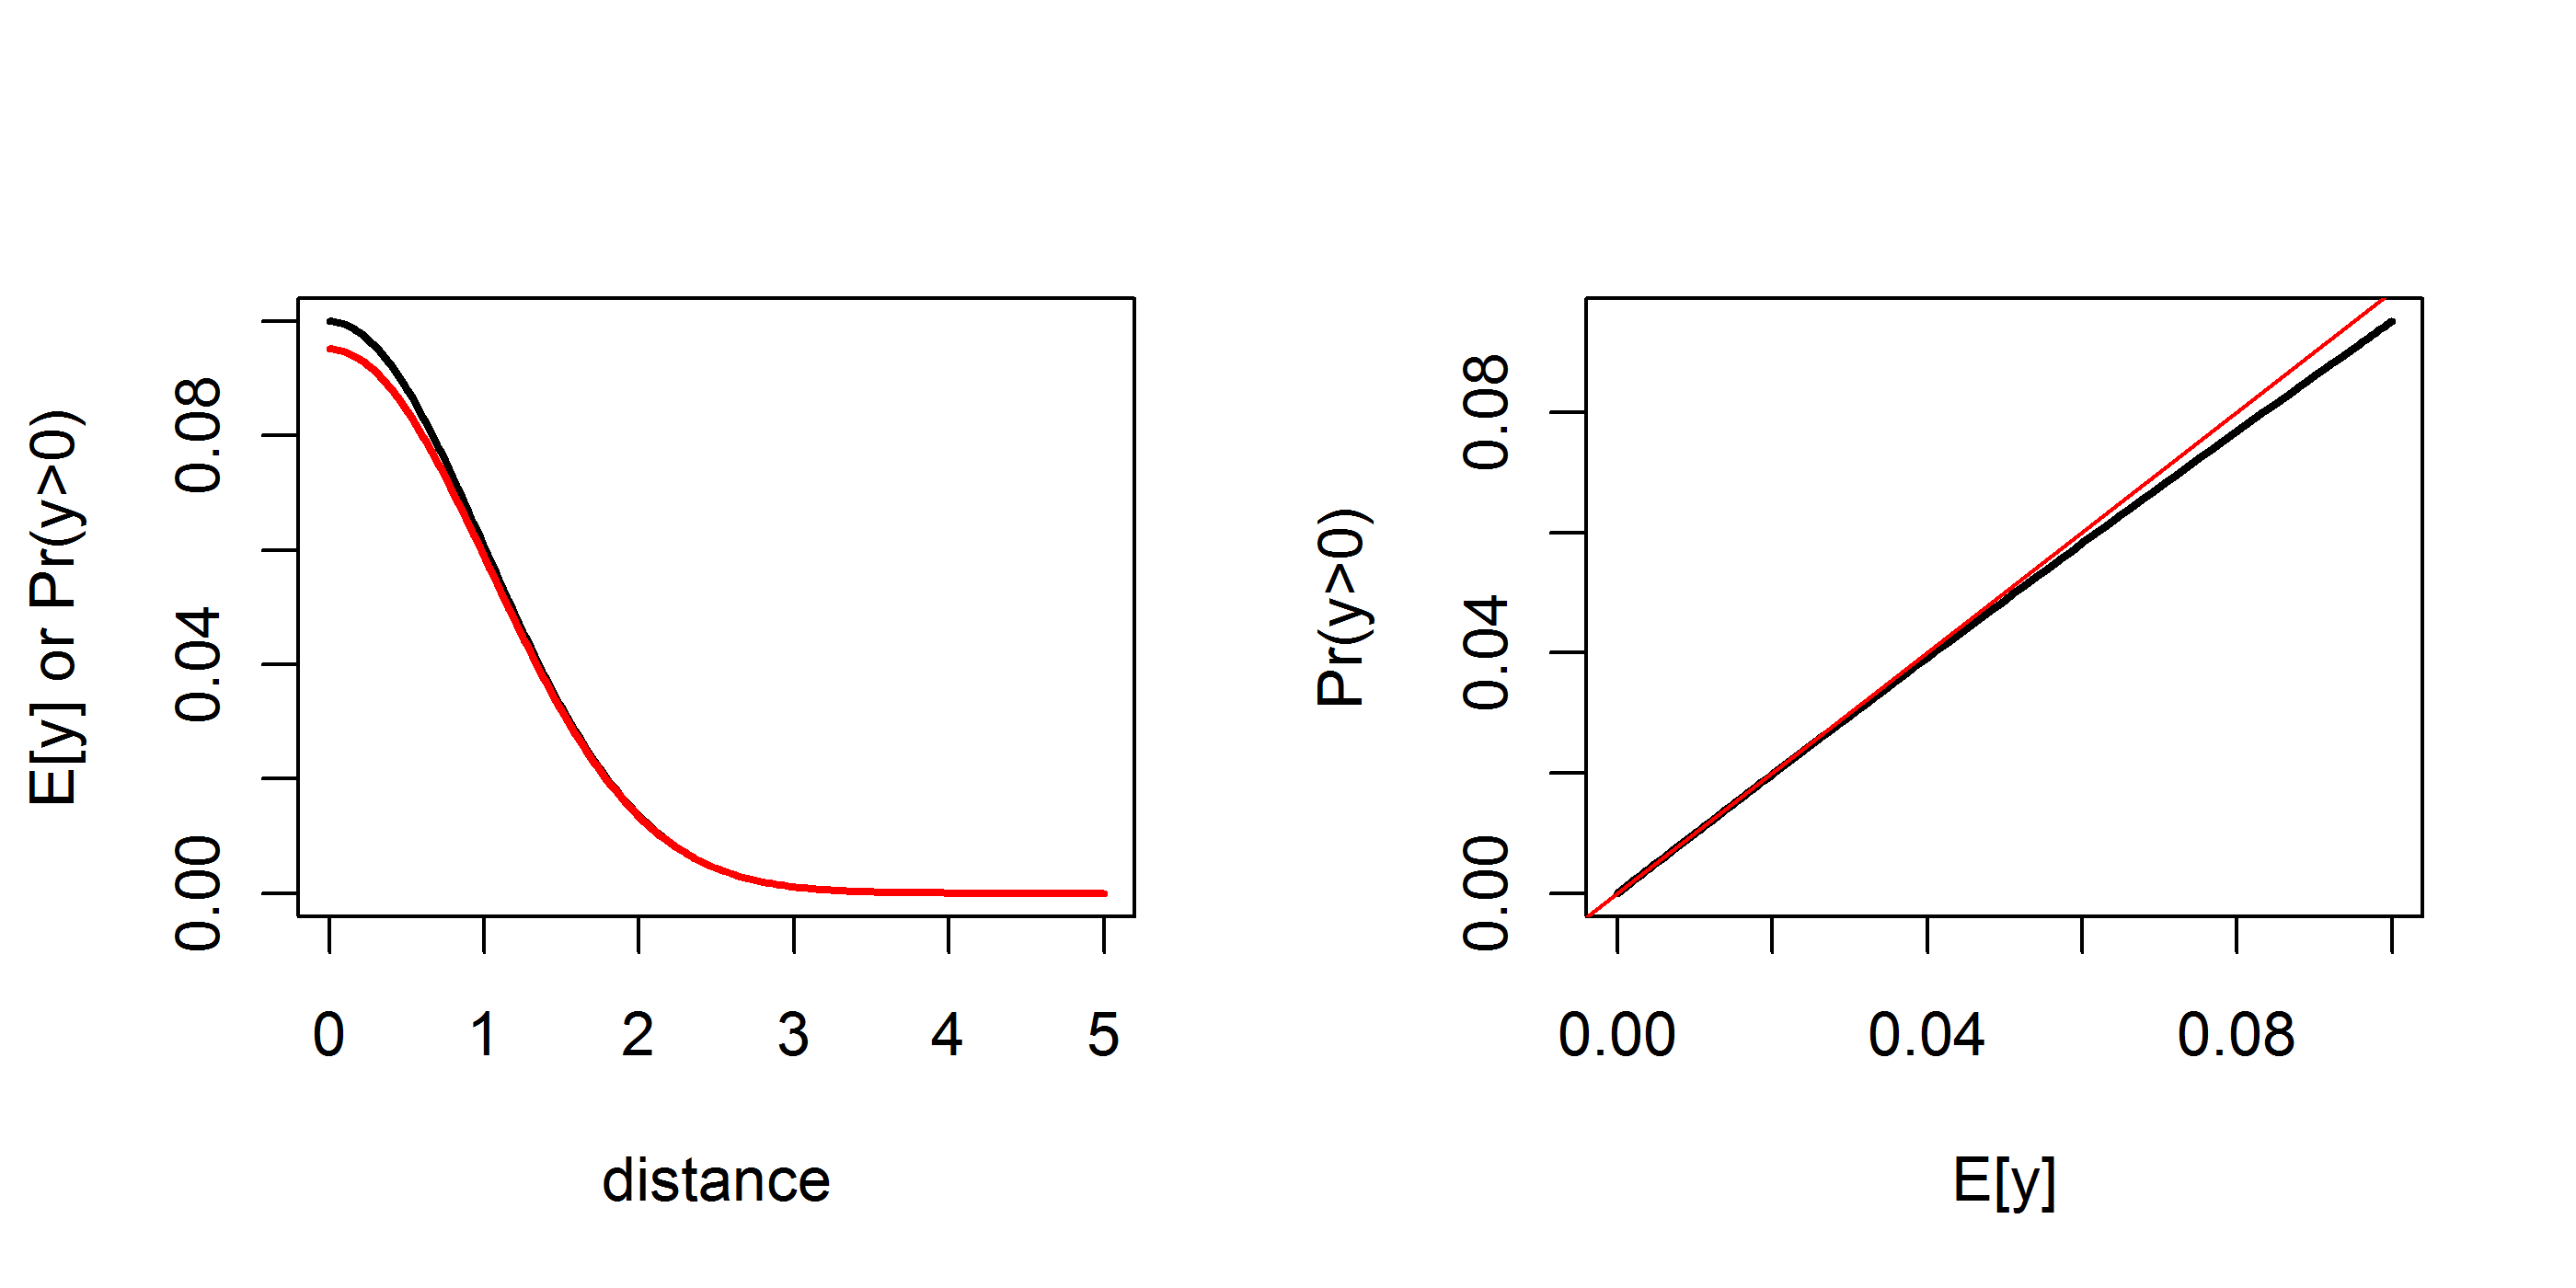
\includegraphics[width=5in,height=2.5in]{Ch9-PoisMn/figs/Poisson-Bern.png}
\caption{
Poisson approximation to the binomial. As the Poisson mean
approaches 0, then $\Pr(y>0)$ under the Poisson model approaches
$\lambda$ and therefore $y \sim \mbox{Poisson}(\lambda)$ is
well-approximated by a Bernoulli model with parameter $\lambda$.  }
\label{poisson-mn.fig.poissonbern}
\end{figure}

Even in such cases
where the Poisson and
Bernoulli models are
not quite
equivalent, we might choose to truncate
individual encounter frequencies to binary observations anyhow
(transforming counts to 0/1 is called ``quantizing'').  We might do
this intentionally in some cases, such as when the distinct encounter events are
highly dependent as often happens in camera trap studies when the same
individual moves back-and-forth in front of a camera during a short
period of time.
But sometimes,
truncation is a feature of the sampling. For example, in the case of
bear hair snares, the number of encounters might be well approximated
by a Poisson distribution but we cannot determine unique visits and so
only get to observe the binary event ``$y>0$''. 
%Similarly for scat
%sampling problems it will not always be possible to diagnose
%distinct ``independent'' scat samples (i.e., due to 
% distinct visits to a location). 
In this case, we might choose to model the encounter probability for
the binary encounter using
 Eq. \ref{poisson-mn.eq.cloglog-inverse}.
This is equivalent to the complementary log-log link model, or the
``Gaussian hazard'' as we called it in Chapt. \ref{chapt.scr0}:
\[
\mbox{ cloglog}(p_{ij}) = \log(\lambda_{0})  + \log(k({\bf x},{\bf s}))
\]
where $\mbox{cloglog}(u) = \log(-\log(1-u))$.
\begin{comment}
This example shows us that the choice of link function is typically
directly related to a specific encounter frequency model and,
furthermore, the choice of link function is equivalent to choice of
``detection function.''
\end{comment}

\subsection{A cautionary note on modeling encounter frequencies}

Other models for counts might be appropriate. For example, ecologists
are especially fond of negative binomial models for count data
\citep{verhoef_boveng:2007,white_bennetts:1996,kery_etal:2005}
but other models for excess-Poisson variation are possible. For
example, we might add a normally distributed random effect to
the linear predictor \citep{coull_agresti:1999}.

As a general rule we favor the Bernoulli observation model even if
our sampling scheme produces encounter frequencies. The main reason is
that, with frequency data, we are forced to confront a model choice
problem (i.e., Poisson, negative binomial, log-normal mixture) that is
wholly unrelated to the fundamental space usage process that underlies
the genesis  % XXXX Again, Borchers might view this as too
             % narrow. i.e. it doesn't fit into his monkey counting
             % problem, or his frog counting using microphones
of many types of SCR data.
Repeated encounters over short time intervals
are not likely to be the result of independent encounter events. E.g.,
an individual moving back and forth in front of a camera yields a
cluster of observations that is not informative about the underlying
spatial structure of the population. Similarly in scat surveys dogs
are used to locate scats which are processed in the lab for
individuality \citep{kohn_etal:1999, mackay_etal:2008,
  thompson_etal:2012}.  The process of local scat deposition is not
strictly the outcome of movement or space usage but rather the outcome
of complex behavioral considerations as well as dependence in
detection of scat by dogs.
For example, dogs find (or smell) one scat and
then are more likely to find one or more nearby ones, if present, or
they get into a den or latrine area and find many scats.  The
additional assumption required to model variation in observed
frequencies (i.e., conditional on location) provides relatively no
information about space usage and density, and we feel that the model
selection issue should therefore be avoided.

To elaborate on this, we suppose that an individual with activity
center ${\bf s}$ visits a
particular pixel ${\bf x}$
% XXXX This notation might confuse people: "an individual s". ie, I think
% we have to be careful when we switch from s being an individual's
% activity center to s being an individual. Same goes for x being the
% location of a trap to x being a pixel.
with some probability $p({\bf x}, {\bf
  s})$, and then, once there, deposits a number of scat, or visits
a camera some number of times with frequency $y({\bf x},{\bf s}) \ge
0$.  We describe the outcome of this movement/usage process with a two-level
hierarchical model of the form: $[y|w][w|p({\bf x},{\bf s})]$ where
$w({\bf x},{\bf s})$ is a binary variable that indicates whether the
individual with activity center ${\bf s}$ used pixel ${\bf x}$
during some interval, and let $w({\bf x},{\bf s}) \sim
\mbox{Bernoulli}(p({\bf x},{\bf s}))$. If we suppose  encounter frequency
$y$ is independent of ${\bf x}$ and ${\bf s}$ conditional on the
use variable  $w$, then  we see that
the model for $y$ (amount of use) does not depend on ${\bf s}$.


\begin{comment}
Moreover, consideration of encounter frequency data could lead to
important identifiability problems along the lines of \citet{link:2003}. The
basic Poisson model can be over-dispersed in a number of ways to
produce different models of over-dispersion.  i.e., gamma noise,
normal noise, exponential noise, etc..  Thus we have different models
of heterogeneity, analogous to the class of models considered by
\citet{link:2003},
\end{comment}

\subsection{Analysis of the Poisson SCR model in BUGS}

We consider the simplest possible model here in which we have no
covariates that vary over sample occasions  $k=1,2,\ldots,K$
so that we work with
the aggregated individual- and trap-specific encounters:
\[
y_{ij} = (\sum_{k=1}^{K} y_{ijk}) =  \mbox{Poisson}(K  \lambda_{0}
k({\bf x}_{j},{\bf s}_{i}) )
\]
and we consider the bivariate normal form of $k({\bf x},{\bf s})$:
\[
k({\bf x},{\bf s}) = \exp( -d({\bf x}, {\bf
  s})^{2} /(2\sigma^{2}))
\]
so that
\[
\log( \lambda_{ij})  =\alpha_{0} - \alpha_{1} d({\bf x}_{j}, {\bf s}_{i})^2
\]
where $\alpha_{0} = \log(\lambda_{0})$ and $\alpha_1 = 1/(2\sigma^2)$.


As usual, we approach Bayesian analysis of these models using data
augmentation (Sec. \ref{closed.sec.da}).  Under data augmentation, we
introduce a collection of all-zero encounter histories to bring the
total size of the data set up to $M$, and a corresponding set of data
augmentation variables $z_{i} \sim \mbox{Bern}(\psi)$. Then the
observation model is specified conditional on $z$ according to:
\[
y_{ij} \sim  \mbox{Poisson}(z_{i} K  \lambda_{ij})
\]
% XXXX Do we want to call the augmented data "yz"?
which evaluates to a point mass at $y=0$ if $z=0$.  In other words,
the observation model under data augmentation is a zero-inflated
Poisson model which is easily analyzed by Bayesian methods, e.g., in
one of the {\bf BUGS} dialects or, alternatively, using likelihood
methods, which we neglect here although the same principles as in
Chapt. \ref{chapt.mle} apply.


\subsection{Simulating data and fitting the model}


Simulating a sample SCR data set under the Poisson model requires only
a couple minor modifications to the procedure we used in
Chapt. \ref{chapt.scr0} (see the function \mbox{\tt simSCR0}). In
particular, we modify the block of code which defines the model to be
that of $\mathbb{E}(y)$ and not $\Pr(y=1)$, and we change the random
variable generator from \mbox{\tt rbinom} to \mbox{\tt rpois}:
\begin{samepage}
{\small
\begin{verbatim}
##
## S =activity centers and traplocs defined as in simSCR0()
##
> D <- e2dist(S,traplocs) # Distance between activity centers and traps

## Define parameter values:
> alpha0 <- -2.5
> sigma <- 0.5
> alpha1 <- 1/(2*sigma*sigma)

## Encounter probability model:
> muy <-  exp(alpha0)*exp(-alpha1*D*D)

## Now generate the encounters of every individual in every trap
> Y <-matrix(NA,nrow=N,ncol=ntraps)
> for(i in 1:nrow(Y)){
    Y[i,] <- rpois(ntraps,K*muy[i,])
  }
\end{verbatim}
}
\end{samepage}

We modified our simulation code from Chapt. \ref{chapt.scr0} to
simulate Poisson encounter frequencies for each trap and then we
analyze an ideal data set using {\bf BUGS}. This Poisson simulator
function {\tt simPoissonSCR} is available in the \mbox{\tt scrbook}
package (it can produce 3-d encounter history data too, although we
don't do that here).  Here is an example of simulating a data set and
harvesting the required data objects, and doing the data augmentation:

\begin{samepage}
{\small
\begin{verbatim}
## Simulate data and extract data elemements
##
> data <- simPoissonSCR(discard0=TRUE,rnd=2013)
> y <- data$Y
> nind <- nrow(y)
> X <- data$traplocs
> K <- data$K
> J <- nrow(X)
> xlim <- data$xlim
> ylim <- data$ylim

## Data augmentation
> M <- 200
> y <- rbind(y,matrix(0,nrow=M-nind,ncol=ncol(y)))
> z <- c(rep(1,nind),rep(0,M-nind))
\end{verbatim}
}
\end{samepage}

The process for fitting
the model in {\bf WinBUGS} or {\bf JAGS} is identical to what we've done
previously in Chapt. \ref{chapt.scr0}. In particular, we set up some
starting values, package the data and inits, identify the parameters
to be monitored, and then send everything off to our MCMC engine. Here
it all is for fitting the Poisson observation model (these commands
are shown in the help file for \mbox{\tt simPoissonSCR}):

{\small
\begin{verbatim}
## Starting values for activity centers
##
> sst <- X[sample(1:J,M,replace=TRUE),] 
> for(i in 1:nind){
  if(sum(y[i,])==0) next
  sst[i,1] <- mean( X[y[i,]>0,1] )
  sst[i,2] <- mean( X[y[i,]>0,2] )
  }
## Dithered a little bit from trap locations
> sst <- sst + runif(nrow(sst)*2,0,1)/8
> data <- list (y=y,X=X,K=K,M=M,J=J,xlim=xlim,ylim=ylim)
> inits <- function(){
   list (alpha0=rnorm(1,-2,.4),alpha1=runif(1,1,2),s=sst,z=z,psi=.5)
   }
> parameters <- c("alpha0","alpha1","N","D")
\end{verbatim}
}
Next, we write the {\bf BUGS} model to an external file:
{\small
\begin{verbatim}
> cat("
model{
 alpha0 ~ dnorm(0,.1)
 alpha1 ~ dnorm(0,.1)
 psi ~ dunif(0,1)

 for(i in 1:M){
   z[i] ~ dbern(psi)
   s[i,1] ~ dunif(xlim[1],xlim[2])
   s[i,2] ~ dunif(ylim[1],ylim[2])
   for(j in 1:J){
      d[i,j] <- pow(pow(s[i,1]-X[j,1],2) + pow(s[i,2]-X[j,2],2),0.5)
      y[i,j] ~ dpois(lam[i,j])
      lam[i,j] <- z[i]*K*exp(alpha0)*exp(- alpha1*d[i,j]*d[i,j])
   }
  }
 N <- sum(z[])
 D <- N/64
}
",file = "SCR-Poisson.txt")
\end{verbatim}
}
To fit the model we execute \mbox{\tt bugs} in the usual way:
{\small
\begin{verbatim}
> library(R2WinBUGS)
> out1 <- bugs (data, inits, parameters, "SCR-Poisson.txt", n.thin=1,
                n.chains=3,n.burnin=1000,n.iter=2000,working.dir=getwd(),
                debug=TRUE)
\end{verbatim}
}
{\flushleft Or, using {\bf JAGS} via \mbox{\tt rjags} we would do
  something like this:}
{\small
\begin{verbatim}
> library(rjags)
> jm <- jags.model("SCR-Poisson.txt", data=data, inits=inits,
                  n.chains=3, n.adapt=1000)
> out2 <- coda.samples(jm, parameters, n.iter=1000, thin=1)
\end{verbatim}
}
{\flushleft
Summarizing } the output from the {\bf WinBUGS}  run produces the following:
{\small
\begin{verbatim}
> print(out1,digits=2)
Inference for Bugs model at "SCR-Poisson.txt", fit using WinBUGS,
 3 chains, each with 2000 iterations (first 1000 discarded)
 n.sims = 3000 iterations saved
           mean    sd   2.5%    25%    50%    75%  97.5% Rhat n.eff
alpha0    -2.57  0.19  -2.95  -2.69  -2.57  -2.44  -2.19 1.00  2600
alpha1     2.34  0.36   1.69   2.08   2.32   2.57   3.12 1.00  3000
N        114.13 15.25  87.97 103.00 113.00 124.00 147.00 1.01   370
D          1.78  0.24   1.37   1.61   1.77   1.94   2.30 1.01   370
deviance 329.95 21.92 290.00 314.20 329.50 344.40 375.80 1.00  1700
...
[..some output deleted..]
...
\end{verbatim}
}

%We don't provide a real example of a Poisson SCR model here although
%we use this observation model for an analysis of some data in Chapt.
%\ref{chapt.searchencounter}. {\bf XXXX DO WE DO THIS ANYWHERE? XXXXX}


\subsection{Analysis of the wolverine study data}

We reanalyzed the data from the wolverine camera trapping study that
were first introduced in Sec. \ref{scr0.sec.wolverine}.  We modified
the {\bf R} script from the function \mbox{\tt wolvSCR0} to fit the
Poisson model (see the help file for \mbox{\tt
  wolvSCR0pois}). Executing this function produces the results shown
in Table \ref{poisson-mn.tab.wolverine}.
\begin{table}
\centering
\caption{Results of fitting the SCR model with Poisson encounter
  frequencies to the wolverine camera trapping data.
Posterior summaries were obtained using {\bf WinBUGS} with
 3 chains, each with 6000 iterations, discarding the first 1000 as
 burn-in, to yield a total of 15000 posterior samples.
}
\begin{tabular}{crrrrrrr} \hline \hline
 Parameter & Mean &  SD & 2.5\% & 50\%  & 97.5\% &Rhat& n.eff \\ \hline
$\psi$     &  0.30& 0.07& 0.19 &  0.30 & 0.45& 1 &  650 \\
$\sigma$   &  0.64& 0.06& 0.54 &  0.64 & 0.76& 1 &  730 \\
$\lambda_{0}$& 0.06& 0.01& 0.04 &  0.06 & 0.08& 1&  5000\\
$\log(p_0)$  &-2.89& 0.17& -3.22& -2.89& -2.57& 1&  5000\\
$N$        & 60.12&11.91& 40.00& 59.00& 87.00& 1&   630\\
$D$        &  5.80& 1.15& 3.86 & 5.69 & 8.39 & 1&   630\\ \hline
%%%$\beta$  & 1.24& 0.21& 0.86 & 1.23 & 1.69 & 1&   730\\
\end{tabular}
\label{poisson-mn.tab.wolverine}
\end{table}
The results are almost indistinguishable from the Bernoulli model
fitted previously, where we had a posterior mean for $N$ of
 $59.84$ and  $\sigma$ was $0.64$. 
You can 
edit the script \mbox{\tt wolvSCR0pois} to  obtain more posterior
 samples, or modify the model in some way.


\subsection{Count detector models in the  \mbox{\tt secr} package}

The {\bf R} package \mbox{\tt secr} will fit Poisson or negative
binomial encounter frequency models. The formatting of data and
structure of the analysis proceeds in a similar fashion to the
Bernoulli model described in Sec. \ref{mle.sec.secr}, except that
we specify the \mbox{\tt detector=``count''} option when the traps
object is created. The set-up proceeds as follows:
\begin{samepage}
{\small
\begin{verbatim}
> library(secr)
> library(scrbook)
> data(wolverine)

> traps <- as.matrix(wolverine$wtraps)
> dimnames(traps) <- list(NULL,c("trapID","x","y",paste("day",1:165,sep="")))
> traps1 <- as.data.frame(traps[,1:3])
> trapfile1 <- read.traps(data=traps1,detector="count")
\end{verbatim}
}
\end{samepage}
You can proceed with analysis of these data and compare/contrast with
the Bayesian analysis given above, or the results of the Bernoulli
model fitted in Chapt. \ref{chapt.mle}.



\section{Independent Multinomial Observations}
\label{poisson-mn.sec.multinomial}

Several types of encounter devices yield multinomial observations in
which an individual can be caught in a single trap during a particular
encounter occasion, but traps might catch any number of individuals.
Mist netting is the canonical example of such a ``multi-catch'' device
\citep{efford_etal:2009euring}. Also some kinds of bird or mammal
cage-traps hold multiple animals, as do pit-fall traps which are
commonly used for many species of herptiles.  Another type of sample
method that might be viewed (in some cases) as a multi-catch device
are area-searches of, for example, reptiles where we think of a small
polygon as the ``trap'' -- we could get multiple individuals (turtles,
lizards) in the same plot but not, in the same sample occasion, at
different plots.  The key features of this independent multinomial or
multi-catch
model are: (1) capture of
an individual in a trap is {\it not} independent of its capture in
other traps, because initial capture precludes capture in any other
trap and (2) individuals behave independently of one another, so
whether a trap captures some individual doesn't have an affect on
whether it captures another.  A type of model in which the 2nd
assumption is violated are the ``single catch'' trap systems which we
address in Sec. \ref{poisson-mn.sec.singlecatch} below. 
 %In general we
 %could imagine some intermediate type of non-independence being 
 %important in any multi-catch
 %situation but, to the best of our knowledge, a general model that
 %encompasses complete dependence (i.e., single-catch) and complete
 %independence (the multinomial model presented here for traditional
 %multi-catch sytems) of individuals has not been proposed.  So
 %we treat the cases individually and, in this section, we address the
 %multi-catch situation wherein individuals behave independently.


In this case we assume the observation ${\bf y}_{ik}$ for individual
$i$ during sample occasion $k$ is a multinomial observation which
consists of a sequence of 0's and  a single 1 indicating the
trap of capture, or ``not captured''. For the ``not captured'' event
we define an additional outcome, by convention element $J+1$ of the
vector.  As an example, if we capture an individual in trap 2 during
some occasion of a study involving $J=6$ traps.
Then, the multinomial observation has length $J+1
= 7$, and the observation is ${\bf y}_{i} = (0,1,0,0,0,0,0)$. An
individual not captured at all would have the observation vector
$(0,0,0,0,0,0,1)$.  If we sample for 5 occasions
in all and the
individual is also caught in trap 4 during occasion 3, but otherwise
uncaptured, then the 5 encounter observations for that individual are
as follows:
% XXXX Suggest emphasizing (again) that column 7 is not a trap, but
% indicates "not captured"
\begin{verbatim}
          occassion  |-------trap -------| "not captured"
                     1   2   3   4   5   6      7
                     ------------------------------------
             1       0   1   0   0   0   0      0
             2       0   0   0   0   0   0      1
             3       0   0   0   1   0   0      0
             4       0   0   0   0   0   0      1
             5       0   0   0   0   0   0      1
\end{verbatim}
Statistically we regard the {\it rows} of this data matrix as {\it
  independent} multinomial trials.

Analogous to our previous Bernoulli and Poisson models, we seek to
construct the multinomial cell probabilities for each individual, as a
function of {\it where} that individual lives, through its center of
activity ${\bf s}$. Thus we suppose that
\begin{equation}
 {\bf y}_{ik}|{\bf s}_{i} \sim \mbox{Multinomial}(1, {\bm \pi}({\bf s}_{i}) )
\label{poisson-mn.eq.mn}
\end{equation}
where ${\bm \pi}({\bf s}_{i})$ is a vector of length $J+1$, where
$\pi_{i,J+1}$, the last cell, corresponds to the probability of the
event ``not captured''.  Now we have to construct these cell
probabilities in some meaningful way that depends on each individual's
${\bf s}$.  We use the standard multinomial logit with distance as a
covariate:
\[
 \pi_{ij} = \frac{  \exp(\alpha_{0} - \alpha_{1} d_{ij}) }{ 1+ \sum_{j}
   \exp(\alpha_{0} - \alpha_{1} d_{ij})}
\]
for $j=1,2,\ldots,J$ and, for $J+1$, i.e., ``not captured'',
\[
 \pi_{i,(J+1)} = \frac{  \exp(0) }
                    { 1+ \sum_{j} \exp(\alpha_{0} - \alpha_{1} d_{ij})}
\]
or, more commonly, we use $d_{ij}^{2}$ to correspond to our Gaussian
kernel model for encounter probability. Whatever function of distance
we use in the construction of multinomial probabilities will have a
direct correspondence to the standard encounter probability models we
used in the Bernoulli or Poisson models as well (see
Sec. \ref{scr0.sec.implied}).

It is convenient to express these multinomial models short-hand as
follows, e.g., for the Gaussian encounter probability model:
\[
\mbox{mlogit}( \pi_{ij} ) = \alpha_{0} - \alpha_{1} d_{ij}^{2}
\]
In this way we can refer to models with covariates in a more concise
way. For example, a model with a trap-specific covariate, say $C_{j}$, is:
\[
\mbox{mlogit}( \pi_{ij} ) = \alpha_{0} - \alpha_{1} d_{ij}^{2} + \alpha_{2} C_{j}
\]
or we could include occasion-specific covariates too, such as
behavioral response.

A statistically equivalent distribution to the multinomial is the {\it
  categorical} distribution.  If ${\bf y}$ is a multinomial trial with
probabilities ${\bm \pi}$ than the {\it position} of the non-zero
element of ${\bf y}$ is a categorical random variable with
probabilities ${\bm \pi}$.  We express this for SCR models as
\[
{\bf y}|{\bf s} \sim \mbox{Categorical}( {\bm \pi}({\bf s})) )
\]
In the SCR context, the categorical version of the multinomial trial
corresponds to the {\it trap of capture}.  Using our example above
with 6 traps then we could as well say $y_{ik}$ is a categorical
random variable with possible outcomes $(1,2,3,4,5,6,7)$ where outcome
$y=7$ corresponds to ``not captured.'' Obviously, how this is
organized or labeled is completely irrelevant, although it is
convenient to use the integers $1$ to $(J+1)$ where $J+1$ is the event
not captured.  Therefore, for our illustration in the previous table,
$y_{i1} = 2$, $y_{i2} = 7$, $y_{i3} = 4$ and so on.

For simulating and fitting data in the {\bf BUGS} engines we will
typically use the categorical representation of the model because it
is somewhat more convenient.  We have found that fitting multinomial
models in {\bf WinBUGS} is less efficient than {\bf JAGS}
\citep{royle_converse:2013}, which we use in the subsequent examples
involving multinomial observation models.


\subsection{Multinomial  resource selection models}

The multinomial probabilities in Eq. \ref{poisson-mn.eq.mnprobs}
look similar to the
multinomial resource selection function (RSF) model for telemetry data
\citep{manly_etal:2002, lele_keim:2006}.  This suggests how we might
model landscape or habitat covariates using such methods -- i.e., by
including them as explicit covariates in a larger multinomial model
for ``use'' -- which, if we take the product of use with encounter,
produces a model for the observable encounter data. This
leads naturally to the development of models that integrate RSF data
from telemetry studies with SCR data
\citep{royle_etal:2012mee},
which is the topic of  Chapt. \ref{chapt.rsf}.



\subsection{Simulating data and analysis using JAGS}

We're going to show the nugget of a simulation function which is
used in the function \mbox{\tt simMnSCR} found in the {\bf R} package
\mbox{\tt scrbook}.  The first lines of the following {\bf R} code
make use of some things that you need to define, but we omit them here
(e.g., \mbox{\tt xlim}, \mbox{\tt ylim} are the boundaries of the
state-space, \mbox{\tt N} is the population size, etc..):
{\small
\begin{verbatim}
##
## Simulate random activity centers:
## (first define N, xlim, ylim, etc..)
##
> S <- cbind(runif(N,xlim[1],xlim[2]),runif(N,ylim[1],ylim[2]))

## Distance from each individual to each trap
> D <- e2dist(S,traplocs)

## Set paramter values
> sigma <- 0.5
> alpha0 <- -1
> alpha1 <- -1/(2*sigma*sigma)

## make an empty data matrix and fill it up with data
> Ycat <- matrix(NA,nrow=N,ncol=K)
>  for(i in 1:N){
    for(k in 1:K){
     lp <- alpha0 + alpha1*D[i,]*D[i,]
     cp <- exp(c(lp,0))
     cp <- cp/sum(cp)
     Ycat[i,k] <- sample(1:(ntraps+1),1,prob=cp)
    }
  }
\end{verbatim}
}
We save the data in the matrix \mbox{\tt Ycat} to clarify that it is
the categorical observation representing ``trap of capture''. 
The matrix \mbox{\tt Ycat} here  has the maximal dimension $N$
and so, to do an  analysis that  mimics a real situation, we would have to
discard the uncaptured individuals.  The function \mbox{\tt
  simMnSCR} in the package \mbox{\tt scrbook} will also simulate
data that includes a behavioral response
%(the parameter
%labeled \mbox{\tt alpha2} shown in the {\bf R} code below),
 which will be the
typical situation in small-mammal trapping problems
\citep[see][for details]{converse_royle:2012}.

Here we use our function \mbox{\tt simMnSCR} to simulate a data set
with $K=7$ occasions.
We'll run the model using \mbox{\tt JAGS}
which we have found is much more effective for this class of models.
We get the data set-up for analysis by augmenting the size of the data
set to $M=200$. In addition we choose starting values for ${\bf s}$
and the data augmentation variables $z$.  For starting values of ${\bf
  s}$ we cheat a little bit here and use the true values for the
observed individuals and then augment the $M \times 2$ matrix ${\bf
  S}$ with $M-n$ randomly selected activity centers. Our function
\mbox{\tt spiderplot} returns the mean observed location of
individuals for use as starting values for the \mbox{\tt nind}
encountered individuals.  The parameters input to
\mbox{\tt simMnSCR} are the intercept $\alpha_{0}$, $\sigma =
\sqrt{1/(2\alpha_{1})}$ for the Gaussian encounter probability model,
and $\alpha_{2}$ is the behavioral response parameter. The data
simulation and set-up proceeds as follows:
{\small
\begin{verbatim}
> set.seed(2013)
> parms <- list(N=100,alpha0= -.40, sigma=0.5, alpha2= 0)
> data <- simMnSCR(parms,K=7,ssbuff=2)
> nind <- nrow(data$Ycat)

> M <- 200
> Ycat <- rbind(data$Ycat,matrix(nrow(data$X)+1,nrow=(M-nind),ncol=data$K))
> Sst <- rbind(data$S,cbind(runif(M-nind,data$xlim[1],data$xlim[2]),
                         runif(M-nind,data$ylim[1],data$ylim[2])))
> zst <- c(rep(1,160),rep(0,40))
\end{verbatim}
}


The model specification is not much more complicated than the binomial
or Poisson models given previously. The main consideration is that we
define the cell probabilities for each trap $j=1,2,\dots,J$ and then
define the last cell probability, $J+1$, for ``not captured'', to be
the complement of the sum of the others. The code is shown in Panel
\ref{poisson-mn.panel.mn}.  In the last lines of code here we specify
$N$ and density, $D$, as derived parameters.

% XXXX Sometimes you use "xlim" and sometimes "Xl" and "Xu". Okay,
% people shouldn't be idiots but there we need to simplify the sea of notation
%% ANDY: RIGHT -- TRYING TO USE/(convert to) "xlim" "ylim" throughout.
\begin{panel}[htp]
\centering
\rule[0.15in]{\textwidth}{.03in}
{\small
\begin{verbatim}
cat("
model {
psi ~ dunif(0,1)
alpha0 ~ dnorm(0,10)
sigma ~dunif(0,10)
alpha1 <-  1/(2*sigma*sigma)

for(i in 1:M){
  z[i] ~ dbern(psi)
  S[i,1] ~ dunif(xlim[1],xlim[2])
  S[i,2] ~ dunif(ylim[1],ylim[2])
  for(j in 1:ntraps){
    #distance from capture to the center of the home range
    d[i,j] <- pow(pow(S[i,1]-X[j,1],2) + pow(S[i,2]-X[j,2],2),1)
  }
  for(k in 1:K){
    for(j in 1:ntraps){
      lp[i,k,j] <- exp(alpha0 - alpha1*d[i,j])*z[i]
      cp[i,k,j] <- lp[i,k,j]/(1+sum(lp[i,k,]))
    }
    cp[i,k,ntraps+1] <- 1-sum(cp[i,k,1:ntraps])  # last cell = not captured
    Ycat[i,k] ~ dcat(cp[i,k,])
  }
}

N <- sum(z[1:M])
A <- ((xlim[2]-xlim[1])*trap.space)*((ylim[2]-ylim[1])*trap.space)
D <- N/A
}
",file="model.txt")

\end{verbatim}
}
\rule[-0.15in]{\textwidth}{.03in}
\caption{
{\bf BUGS} model specification for the independent multinomial
observation model. For data simulation and model fitting see the
help file \mbox{\tt ?simMnSCR} in the {\bf R} package \mbox{\tt scrbook}.
}
\label{poisson-mn.panel.mn}
\end{panel}

To fit the model, we need to package everything up (inits, parameters,
data) and send it off to \mbox{\bf JAGS} to build an MCMC simulator
for us (these commands are executed in the help file for \mbox{\tt
  simMnSCR}). In addition to the usual data objects, we also pass
the limits of the assumed rectangular state-space (\mbox{\tt ylim},
\mbox{\tt xlim}, both $1 \times 2$ vectors) and the scale of the
standardized units, called \mbox{\tt trap.space} here because we
typically will define the trap coordinates to be an integer grid. If
the trap spacing is 10 $m$ and we want units of density computed in
terms of individuals  per {\it meter}-squared, then we input \mbox{\tt
  trap.space=10}. The analysis is carried out as follows:
\begin{samepage}
{\small
\begin{verbatim}
> inits <- function(){  list (z=zst,sigma=runif(1,.5,1) ,S=Sst) }

# parameters to monitor
> parameters <- c("psi","alpha0","alpha1","sigma","N","D")

# bundle the data. Note this reuses "data"
> data <- list (X=data$X,K=data$K, trap.space=1,Ycat=Ycat,M=M,
               ntraps=nrow(data$X),ylim=data$ylim,xlim=data$xlim)

> library(R2jags)
> out <- jags (data, inits, parameters, "model.txt", n.thin=1,
               n.chains=3, n.burnin=1000, n.iter=2000)
\end{verbatim}
}
\end{samepage}

The posterior summaries are provided in the following {\bf R}
output (recall that
$N=100$, $\alpha_{0}= -.40$, and $\sigma=0.5$):
{\small
\begin{verbatim}
> out
Inference for Bugs model at "model.txt", fit using jags,
 3 chains, each with 2000 iterations (first 1000 discarded)
 n.sims = 3000 iterations saved
         mu.vect sd.vect    2.5%     25%     50%     75%   97.5%  Rhat n.eff
D          1.873   0.189   1.531   1.750   1.859   2.000   2.250 1.006  1300
N        119.867  12.107  98.000 112.000 119.000 128.000 144.000 1.006  1300
alpha0    -0.435   0.151  -0.738  -0.535  -0.439  -0.331  -0.146 1.004   580
alpha1     2.195   0.286   1.658   2.004   2.180   2.372   2.785 1.003  2400
psi        0.599   0.069   0.465   0.552   0.599   0.645   0.739 1.006  1400
sigma      0.480   0.032   0.424   0.459   0.479   0.500   0.549 1.003  2400
deviance 892.164  21.988 850.922 877.417 891.561 906.246 937.728 1.003   950

[... output deleted ....]
\end{verbatim}
}


\subsection{Multinomial relationship to the Poisson}

The multinomial is related to the Poisson encounter rate
model by a conditioning argument. Let $y_{ij}$ be the number of
encounters for individual $i$ in trap $j$. If $y_{ij} \sim
\mbox{Poisson}(\lambda_{ij})$,
then,
conditional on the {\it total}
number of captures (i.e., across all traps), $y_{i} = \sum_{j}
y_{ij}$, the trap encounter frequencies are multinomial with
probabilities
\[
 \pi_{ij} =  \frac{ \lambda_{ij} } { \sum_{j} \lambda_{ij} }
\]
for $j=1,2,\ldots,J$.
Or equivalently the {\it trap of
  capture} is categorical with probabilities $\pi_{ij}$ as given above.
Under the Gaussian kernel model, these probabilities are:
\begin{equation}
\pi_{ij} =  \frac{ \exp(  -\alpha_{1}  d({\bf x}_{i},{\bf s}_{i})^2 ) }  {
   \sum_{j} \exp( -\alpha_{1} d({\bf x}_{i},{\bf s}_{i})^2)}
\label{poisson-mn.eq.mnprobs}
\end{equation}
where, we note, the intercept $\alpha_{0}$ has canceled from both the
numerator and denominator. This makes sense because, here, these
probabilities describe the trap-specific capture probabilities {\it
  conditional on capture}.  Therefore, the model is not completely
specified, absent a model for the ``overall'' probability of encounter
or the expected frequency of captures, say $\phi_{i}$. Depending on
how we specify a model for this quantity $\phi_{i}$, we can reconcile
it directly with the Poisson model.
% or the Bernoulli model of
%Chapt. \ref{chapt.scr0}.
Let $y_{i.}$ be the total number of encounters for individual $i$ and
suppose $y_{i.}$ has a Poisson distribution with mean $\phi_{i}$.
Then, marginalizing Eq. \ref{poisson-mn.eq.mn} over the Poisson
distribution for $y_{i.}$ produces the original set of
$iid$ % XXXX I have been using "i.i.d." Should I change to $iid$?
Poisson
frequencies with probabilities:
\[
 \lambda_{ij} = \phi_{i} \pi_{ij}
\]
for $j=1,2,\ldots,J$.
In particular, if we suppose that
$\phi_{i} = \sum_{j} \exp(\alpha_{0} - \alpha_{1} d({\bf x},{\bf s})^2)$
then the marginal distribution of $y_{ij}$ is Poisson with mean $\exp(
\alpha_{0} - \alpha_{1} d({\bf x},{\bf s})^2 )$, equivalent to
Eq. \ref{poisson-mn.eq.lp}.
%An alternative choice of $\phi_{i}$ under the assumption that $y_{i}$ is
%binomial will produce individual- and trap-specific probabilities
%consistent with the binomial model SCR0.
\begin{comment}
  Suppose, instead, that $y_{i}$ is Binomial with sample size $K$ and
  probability $\phi_{i}$. How should we parameterize $\phi_{i}$?  One
  possibility is
\[
\phi_{i} = \lambda_{0} \exp(-\alpha_{1} \sum_{j} d_{ij}^2)
\]
%this is not unnatural we can think of hazard to capture in each trap
%as independent and then sum up the hazards and this is (the
%complement) of the ``mortality function''.
\end{comment}

In summary, the Poisson and multinomial models are equivalent in how
they model the distribution of captures among traps.
 It stands to reason that, if the encounter
rate of individuals is low, we could use the Poisson and multinomial
models interchangeably. In fact, based on our discussion in Sec.
\ref{poisson-mn.sec.approx}
above we could use any of the binomial/Poisson/multinomial models with
little ill-effect when encounter rate is low.



%So we can think of this multinomial model as arising naturally
%by having Poiosson encounters and then conditioning on the total.
%It is a sensible model to have anyhow, as it just allocates captures
%to traps in proportion to the square of distance.  We could try other
%models here too (Note: What do Borchers and Efford 2008 do?).

%People might think this multinomioal model is somehow more general
%than assuming Poisson encounter frequencies since we might cook up the
%multinomioal without having to specify a distribution for
%$y_{i}$. That said, we note that it arises under
%If we now uncondition on the total.....
%$y_{ij}$ is Poisson with mean $\sum_{j}$ stuff... we have a product of
%Poissons, i.e., the model we started with.

\begin{comment}
The interpretation of this formulation of the multinomial model merits
some discussion. That is, {\it given that an individual is captured},
the probabilities given by Eq. \ref{poisson-mn.eq.mnprobs} determine
the probability distribution of ``trap of capture''.  The probability
that individual $i$ is captured in trap $j$ is the product of two
components
\[
\pi_{ij} = \Pr(\mbox{individual} i \mbox{captured in trap} j) =
 \Pr(\mbox{captured in trap} j | \mbox{captured at all})\Pr(\mbox{captured at all})
\]
To fully specify the model, we have to model the probability that an
individual is captured at all, say $p_0$. Then the unconditional
multinomial probabilities are $p_{0} \pi_{ij}$ for $j=1,\ldots,J$ and
$\pi_{i,J+1} = (1-p_{0})$.  It hardly makes sense that $p_{0}$ should
be constant.  Instead, it is natural to think that total probability
of capture should be related to the average distance to traps like
this:
\[
 p_{i} = p_{0} \exp(-\beta \sum_{j} D_{ij}^2)
\]
the argument to justify this is that the total hazard to capture, if
traps function independently, is the sum of that due to each trap, i.e.,
\[
 h_{i} = \sum_{j} h_{ij}
\]
so we set $h_{ij} = \propto D_{ij}^{2}$ which I think is the Gompertz
hazard model.
%Then
%the the survival function $S=exp(-H)$ so we equate $p$ to ``survival'' (hardly makes sense
%but, hey, thats the model that people use).
Then we have the marginal probability of capture in trap $j$ is
(multiplying $p_{i}$ with $\pi_{ij}$):
\[
\pi_{ij} =   p_{0}  \exp(-\beta D_{ij}^2)
\]
and then the probability of not being captured at all is
\[
 \pi_{i,J+1} =  1-p_i
\]
Therefore the multinomial trial ${\bf y}_{i}$ of length  $(J+1)
XXXX problem here -- do those add up to 1? XXXXX
XXX
\times 1$ has those probabilities.  One issue: This induces a
constraint on $p_{0}$ because the sum of the multinomial probabilities
has to be 1 and therefore
\[
p_{0} \sum_{j} p_{ij} \le 1.
\]
References to Royle et al. 2009a and Gardner et al. 2010 need to go
here because those papers used this type of model. (misspecified
multinomial).
This is not the ``multivariate logit'' that
we use in the BUGS model above which more naturally admits the
restriction on the cell probabilities, see Eq. XXXX above.


In summary, there is a coherent linkage between the Poisson,
multinomial, and the Binomial model. If trap-level encounter
histories are $iid$ Poisson random variables with $\lambda_{ij} =
\lambda_{0}exp(-\alpha_{1} d^{2})$, then the trap-of-capture,
conditional on the total number of captures, has a multinomial
distribution with cell probabilities $\pi_{ij} =
\lambda_{ij}/(\sum_{j} \lambda_{ij})$ and then if the hazard to
capture is proportion to $d^{2}$, and the traps are independent, then
$\pi_{ij} = p_{0} exp(-\alpha_{1} d_{ij}^{2})$ with a restriction on
$p_{0}$.  So those models are all
equivalent to some extent, for their appropriate observation model.

\end{comment}



\subsection{Avian mist-netting example}
\label{poisson-mn.sec.ovenbird}

We analyze data from a mist-netting study of ovenbirds, conducted at
the Patuxent Wildlife Research Center, Laurel MD, by D.K. Dawson and M.G.
Efford. The data from this study are available in the \mbox{\tt secr}
package, and have been analyzed previously by
\citet{efford_etal:2004}, see also \citet{borchers_efford:2008}.
Forty-four mist nets spaced 30 m apart on the perimeter of a 600-m x
100-m rectangle were operated on 9 or 10 non-consecutive days in late
May and June for 5 years from 2005-2009.  
%From the \mbox{\tt secr}
%documentation of this data set we take this:
%\begin{quote}
%{\it
%  Netting was passive (i.e. song playback was not used to lure birds
%  into the nets). Birds received individually numbered bands, and both
%  newly banded and previously banded birds were released at the net
%  where captured. Sex was determined in the hand from the presence of
%  a brood patch (females) or cloacal protuberance (males).}
%\end{quote}
The ovenbird
data can be loaded as follows:
\begin{verbatim}
> library(secr)
> data(ovenbird)
\end{verbatim}
The dataset consists of adult ovenbirds caught during sampling in each
of 5 years, 2005-2009. (one ovenbird was killed in 2009, indicated by
a negative net number in the encounter data file).
As with most mist-netting studies, nets are checked multiple times
during a day (e.g., every hour during a morning session). However, for
this data set, the within-day recaptures are not included so each bird
has at most a single capture per day. Therefore the multinomial model
(detector type `multi' in \mbox{\tt secr}) is appropriate.
 Although
several individuals were captured in more than one year, this
information is not used in the models presently offered in \mbox{\tt
  secr}, but we do make use of it in the development of open models in
Chapt. \ref{chapt.open}.
%
%{\it
%  An analysis of the data for males in the first four years showed
%  that they tended to avoid nets after their first capture within a
%  season (Dawson and Efford 2009). While the species was present
%  consistently, the number of detections in any one year was too small
%  to give reliable estimates of density; pooling of detection
%  parameters across years helped to improve precision.
%}


\subsubsection{Multiple sample sessions}

Up to this point we have only dealt with a basic closed population
sampling situation consisting of repeated sample occasions on a single
population of individuals using a single array of traps. In practice,
many studies produce repeated samples over longer periods of time over
which demographic closure isn't valid, or at different
locations where the populations are completely distinct. We adopt the \mbox{\tt secr} terminology of {\it session}
for such replication by groups of time or space, and the models are
{\it multi-session} models, although we think of such models as being
relevant to any stratified population (see Chapt. \ref{chapt.hscr}).
We introduced \mbox{\tt secr}'s
multi-session models in Sec. \ref{mle.sec.multisession}.  In the case
of the ovenbird data, sampling was carried out in multiple years, with
a number of sample occasions within each year (9 or 10), a type of
data structure commonly referred to as ``the robust
design'' \citep{pollock:1982}.  In this context,
it stands to reason that there is recruitment and mortality happening
across years. In Chapt. \ref{chapt.open} we model these processes
explicitly but, here, we provide an analysis of the data that does not
require explicit models for recruitment and survival, regarding the
yearly populations as independent strata, and fitting a multi-session
model.

When the sessions represent explicit time periods,
the multi-session model of \mbox{\tt secr} 
can be thought of as a type of open population model. 
In particular, a special case of open models arises when
we assume $N_{t}$ (time-specific population sizes) are independent
from one time period or session to the next -- this can be thought of
as a ``random temporary emigration'' model of the
\citet{kendall_etal:1997} variety, and this is the 
multi-session model implemented in \mbox{\tt secr}.  In particular, by
assuming that $N_{t}$ is Poisson with mean $\Lambda_{t}$, one can model
variation in abundance among sessions based on the Poisson-integrated
likelihood in which parameters of $\Lambda_{t}$ appear directly in the
likelihood as we noted in Sec. \ref{mle.sec.multisession}.  We provide
an analysis (below) of the ovenbird data here using the multi-session
models in \mbox{\tt secr}.  We formalize the multi-session model
approach from a Bayesian perspective using data augmentation in
Chapt. \ref{chapt.hscr} \citep{converse_royle:2012,royle_converse:2013}.

A 3rd way to develop models for stratified or grouped populations, not
based on multi-session models, but that is convenient in {\bf BUGS},
is to regard the data from each session as an independent data set
with its own $N_{t}$ parameter, and do $T$ distinct data
augmentations. Because each $N_{t}$ is regarded as a free parameter,
independent of the other parameters, we'll call this the nonparametric
multi-session model to distinguish it from the multi-session model
which assumes the $N_{t}$ are related to one another by having been
generated from a common Poisson distribution.  We can analyze this
model in the normal context of data augmentation by augmenting each
year separately in the same {\bf BUGS} model specification. This
approach avoids making explicit model assumptions about the $N_{t}$
parameters.  This is distinct from the model implemented in \mbox{\tt
  secr} in that \mbox{\tt secr} is removing the $N_{t}$ parameters by
integrating the conditional-on-$N_{t}$ likelihood over the Poisson
prior for $N_{t}$\footnote{We do not know of \mbox{\tt secr}
  documentation that states this (or contradicts it). We think this is
  what is being done, based partially on conversations or emails with
M.G. Efford,   D.L. Borchers, the various publications on \mbox{\tt
  secr}, and thinking about it.}
% XXXX Are you sure that this is what secr is doing? Where is the
% documentation explaining how secr fits multi-session models? They
% never actually sum over all possible values of N, right?

We
demonstrate these 3  approaches to analyzing grouped/stratified data
using the ovenbird data: (1) In the
following section, we provide the nonparametric multi-session model with
unconstrained $N_{t}$; (2) we demonstrate  the Poisson model-based
multi-session models from \mbox{\tt secr} both here (following section) and in
Chapt. \ref{chapt.hscr} from a Bayesian standpoint; (3) 
later, in Chapt. \ref{chapt.open}, we provide a fully dynamic  ``spatial Jolly-Seber''
model and apply it to the ovenbird data.


\subsubsection{Analysis in JAGS}

The ovenbird data are provided as a multi-session \mbox{\tt capthist}
object \mbox{\tt ovenCH} which, by regarding years as independent
strata, or sessions, allows for the fitting of the multi-session model.  For doing
a Bayesian analysis in one of the {\bf BUGS} engines (we use {\bf
  JAGS} here) there are a number of ways to structure the data and
describe the model.  We can analyze either a 2-d data set with all
years (data augmented) ``stacked'' into a data set of dimension $(5*M)
\times 10$ (5 years, $M=$ size of the augmented data set, $K=10$
replicate sample occasions). Or, we could produce a 3-d array ($M \times J
\times K$). We adopted the former approach, analyzing the data as a
2-d array and creating an additional categorical  variable for ``year''
to indicate which stratum (year) each record goes with.  There was a
single loss-on-capture which we accounted for by fixing $p=0$ for all
subsequent encounters of that individual (indicated by the binary
variable \mbox{\tt dead}, as shown in Panel
\ref{poisson-mn.panel.ovenbird}).  We have an {\bf R} script in
\mbox{\tt scrbook} package called \mbox{\tt SCRovenbird}, so you can
see how to set-up the data and run the model.  Executing the script
\mbox{\tt SCRovenbird} produces the posterior summaries given in Table
\ref{scrovenbird.results}. Here, density is in units of birds per ha.


Data on individual sex is included
with \mbox{\tt secr}, but  we provide an analysis of a single model
for all adults, constant $\sigma$ across years, constant $p_{0}$, and
year-specific values of $N_{t}$ (and hence $D_{t}$).
 There is a habitat mask provided with the data but the mask
appears to just be a modified rectangle around the net locations,
clipped to have rounded corners, and so we don't use it here.






\begin{panel}[htp]
\centering
\rule[0.15in]{\textwidth}{.03in}
%\begin{minipage}{2.5in}
{\small
\begin{verbatim}
model{
 alpha0 ~ dnorm(0,.1)
 sigma ~ dunif(0,200)
 alpha1 <- 1/(2*sigma*sigma)

 A <- ((xlim[2]-xlim[1]))*((ylim[2]-ylim[1]))
 for(t in 1:5){
  N[t] <- inprod(z[1:bigM],yrdummy[,t])
  D[t] <- (N[t]/A)*10000  # put in units of per ha
  psi[t] ~ dunif(0,1)
 }

 for(i in 1:bigM){  # bigM = total size of jointly augmented data set
   z[i] ~ dbern(psi[year[i]])
   S[i,1] ~ dunif(xlim[1],xlim[2])
   S[i,2] ~ dunif(ylim[1],ylim[2])

 for(j in 1:ntraps){  # X = trap locations, S = activity centers
    d2[i,j] <- pow(pow(S[i,1]-X[j,1],2) + pow(S[i,2]-X[j,2],2),1)
  }
 for(k in 1:K){
   Ycat[i,k] ~ dcat(cp[i,k,])
   for(j in 1:ntraps){
     lp[i,k,j] <- exp(alpha0 - alpha1*d2[i,j])*z[i]*(1-dead[i,k])
     cp[i,k,j] <- lp[i,k,j]/(1+sum(lp[i,k,1:ntraps]))
   }
   cp[i,k,ntraps+1] <- 1-sum(cp[i,k,1:ntraps])  # last cell = not captured
  } 
 }  
}
\end{verbatim}
}
%\end{minipage}
\rule[-0.15in]{\textwidth}{.03in}
\caption{
{\bf BUGS} model specification for the non-parametric multi-session
model in which each $N_{t}$ is independent of the other. The implied
prior (by data augmentation) is that $N_{t} \sim
\mbox{Uniform}(0,100)$.
To fit this model to the ovenbird data, see
 \mbox{\tt ?SCRovenbird} in the {\bf R} package \mbox{\tt scrbook}.
}
\label{poisson-mn.panel.ovenbird}
\end{panel}


\begin{table}[t!]
\centering
  \small
  \caption{Posterior summary statistics
for the ovenbird mist-netting data based on the
    independent multinomial (``multi-catch'') encounter process
    model. Parameters $\psi$, $N$ and $D$ are indexed by year.
MCMC was done using
    {\tt jags} with 3 chains, each with 5000 iterations, discarding
    the first 1000, for a total of 12000 posterior samples.}
  \begin{tabular}[t]{crrrrrrr}
    \hline \hline
parameter   &  Mean &  SD &  2.5\%  &  50\%  &  97.5\%  & Rhat &  n.eff \\
    \hline
D[1]  &   1.000 &  0.202&  0.682&  0.971&  1.446& 1.009 &  250\\
D[2]  &   1.041 &  0.192&  0.723&  1.033&  1.467& 1.010 &  230\\
D[3]  &   1.212 &  0.208&  0.868&  1.198&  1.653& 1.004 &  580\\
D[4]  &   0.895 &  0.173&  0.599&  0.868&  1.281& 1.012 &  190\\
D[5]  &   0.760 &  0.155&  0.496&  0.744&  1.095& 1.002 & 1700\\
$\alpha_0$&  -3.488 &  0.159& -3.801& -3.490& -3.171& 1.005 &  450 \\
$\alpha_1$&   0.000 &  0.000&  0.000&  0.000&  0.000& 1.018 &  120 \\
$\sigma$ &  76.106 &  6.061& 65.620& 75.709& 89.205& 1.018 &  120\\
$\psi[1]$&   0.484 &  0.108&  0.299&  0.475&  0.715& 1.008 &  300\\
$\psi[2]$&  0.505 &  0.103&  0.325&  0.497&  0.725& 1.008 &  270\\
$\psi[3]$&   0.585 &  0.110&  0.388&  0.578&  0.813& 1.004 &  710\\
$\psi[4]$&   0.434 &  0.095&  0.264&  0.428&  0.639& 1.010 &  210\\
$\psi[5]$&   0.370 &  0.087&  0.215&  0.364&  0.556& 1.002 & 2000\\
N[1]  &  48.396 &  9.762& 33.000& 47.000& 70.000& 1.009 &  250\\
N[2]  &  50.403 &  9.290& 35.000& 50.000& 71.000& 1.010 &  230\\
N[3]  &  58.687 & 10.049& 42.000& 58.000& 80.000& 1.004 &  580\\
N[4]  &  43.341 &  8.366& 29.000& 42.000& 62.000& 1.012 &  190\\
N[5]  &  36.792 &  7.502& 24.000& 36.000& 53.000& 1.002 & 1700\\
\hline
  \end{tabular}
  \label{scrovenbird.results}
\end {table}




\subsubsection{Analysis in \mbox{\tt secr} }


Included with the ovenbird data are a number of  models fitted as
examples. Those include:
{\small
\begin{verbatim}
ovenbird.model.1   fitted secr model -- null
ovenbird.model.1b  fitted secr model -- g0 net shyness
ovenbird.model.1T  fitted secr model -- g0 time trend within years
ovenbird.model.h2  fitted secr model -- g0 finite mixture
ovenbird.model.D   fitted secr model -- trend in density across years
\end{verbatim}
}
The model fit objects provided in \mbox{\tt secr} are based on the use
of the habitat mask.
To make the analyses consistent with our previous analysis in {\bf
  JAGS}, we 
refit all of the models here without the habitat mask.
The re-analysis proceeds as follows:
{\small
\begin{verbatim}
## fit constant-density model
> ovenbird.model.1 <- secr.fit(ovenCH)
## fit net avoidance model
> ovenbird.model.1b <- secr.fit(ovenCH, model =   list(g0 ~ b))
## fit model with time trend in detection
> ovenbird.model.1T <- secr.fit(ovenCH, model =    list(g0 ~ T))
## fit model with 2-class mixture for g0
> ovenbird.model.h2 <- secr.fit(ovenCH, model =    list(g0 ~ h2))
## fit a model with session (year)-specific Density
> ovenbird.model.D <- secr.fit(ovenCH, model =    list(D ~ session))
\end{verbatim}
}
All of these can be fitted easily in {\bf JAGS} but
the model we fitted was roughly equivalent to the last model,
\mbox{\tt ovenbird.model.D}, because we allowed for year-specific
population sizes (and hence density). So, we'll
compare our results from {\bf JAGS} to that
model.  We ran that model with \mbox{\tt buffer=300}. For values of
200 or less,  \mbox{\tt
  secr} throws a bias warning message at us.
The \mbox{\tt secr} 
output is extensive 
and so we
do not reproduce it completely here. By default, it summarizes the
trap information for each year, encounter information, and then output for
each year. Here is an abbreviated version for \mbox{\tt ovenbird.model.D}:
{\small
\begin{verbatim}

> print(ovenbird.model.D,digits=2)

secr.fit( capthist = ovenCH, model = list(D ~ session), buffer = 300 )
secr 2.3.1, 14:46:52 23 Jan 2013

$`2005`
Object class      traps 
Detector type     multi 
Detector number   44 
Average spacing   30.27273 m 
x-range           -50 49 m 
y-range           -285 285 m 

[... deleted ...]

           2005 2006 2007 2008 2009
Occasions     9   10   10   10   10
Detections   35   42   52   30   33
Animals      20   22   26   19   16
Detectors    44   44   44   44   44

Model           :  D~session g0~1 sigma~1 
Fixed (real)    :  none 
Detection fn    :  halfnormal 
Distribution    :  poisson 
N parameters    :  7 
Log likelihood  :  -1119.845 
AIC             :  2253.689 
AICc            :  2254.868 

[... deleted ...]
\end{verbatim}
}

To do model selection  we use the handy helper-function \mbox{\tt AIC}
as follows (output edited to fit on the page):
{\small
\begin{verbatim}
[trash these]
 AIC (ovenbird.model.1, ovenbird.model.1b, ovenbird.model.1T,
     ovenbird.model.h2,ovenbird.model.DT)

                   model  detectfn npar logLik    AIC     AICc     dAICc 
ovenbird.model.1T  [edited output]  4 -1113.429 2234.858 2235.266  0.000 
ovenbird.model.1b      ....         4 -1120.161 2248.323 2248.731 13.465 
ovenbird.model.h2      ....         5 -1119.337 2248.674 2249.293 14.027 
ovenbird.model.1       ....         3 -1122.650 2251.299 2251.542 16.276 
ovenbird.model.DT      ....         7 -1121.331 2256.662 2257.841 22.575 



new results: 
> ## compare & average pre-fitted models
> AIC (ovenbird.model.1, ovenbird.model.1b, ovenbird.model.1T,
+     ovenbird.model.h2,ovenbird.model.D)
                                      model   detectfn npar    logLik      AIC     AICc  dAICc AICwt
ovenbird.model.1T          D~1 g0~T sigma~1 halfnormal    4 -1111.850 2231.700 2232.109  0.000     1
ovenbird.model.1b          D~1 g0~b sigma~1 halfnormal    4 -1117.615 2243.229 2243.637 11.528     0
ovenbird.model.1           D~1 g0~1 sigma~1 halfnormal    3 -1121.164 2248.327 2248.570 16.461     0
ovenbird.model.h2 D~1 g0~h2 sigma~1 pmix~h2 halfnormal    5 -1119.762 2249.524 2250.143 18.034     0
ovenbird.model.D     D~session g0~1 sigma~1 halfnormal    7 -1119.845 2253.689 2254.868 22.759     0
> 

\end{verbatim}
}
We see that the null model is way down at the bottom of the list, just
ahead of the model 
with year-specific density. Instead, 
the model with a time-trend (within-season) in detection probability
is preferred, followed by a behavioral response. We encourage you to
adapt the {\bf JAGS} model specification for such models which is easily
done (see Chapt. \ref{chapt.covariates} for many examples).
We provide the summary results for the model having \mbox{\tt D $\sim$
  session} as follows:
{\small
\begin{verbatim}
Results for "D[session]" model:


> print(ovenbird.model.D.300,digits=2)

secr.fit( capthist = ovenCH, model = list(D ~ session), buffer = 300 )
secr 2.3.1, 14:46:52 23 Jan 2013

[...deleted....]

Fitted (real) parameters evaluated at base levels of covariates 

 session = 2005 
       link estimate SE.estimate    lcl    ucl
D       log    0.920       0.228  0.571  1.484
g0    logit    0.028       0.004  0.021  0.037
sigma   log   78.566       6.379 67.025 92.095

 session = 2006 
       link estimate SE.estimate    lcl    ucl
D       log    0.963       0.238  0.598  1.553
g0    logit    0.028       0.004  0.021  0.037
sigma   log   78.566       6.379 67.025 92.095

 session = 2007 
       link estimate SE.estimate    lcl    ucl
D       log    1.139       0.282  0.706  1.836
g0    logit    0.028       0.004  0.021  0.037
sigma   log   78.566       6.379 67.025 92.095

 session = 2008 
       link estimate SE.estimate    lcl    ucl
D       log    0.832       0.206  0.516  1.341
g0    logit    0.028       0.004  0.021  0.037
sigma   log   78.566       6.379 67.025 92.095

 session = 2009 
       link estimate SE.estimate    lcl    ucl
D       log    0.701       0.173  0.435  1.130
g0    logit    0.028       0.004  0.021  0.037
sigma   log   78.566       6.379 67.025 92.095
\end{verbatim}
}
The point estimates (MLEs) of density are uniformly lower than the Bayesian estimates
(posterior means)
shown in Table \ref{scrovenbird.results}.
We expect some difference in this direction due to
small-sample skew of the posterior, although for year 2 and 3 the
difference is even in the opposite relative direction which is
surprising\footnote{This difference between the \mbox{\tt secr} and \mbox{\bf
  JAGS} results is possibly due to the fact that the \mbox{\tt secr}
multi-session 
model assumes that the $N_{t}$ have a Poisson distribution but the
implementation in {\bf JAGS} using data augmentation is based on a
binomial model.}.
The estimated $\sigma$ is very similar between the {\bf JAGS}
analysis and \mbox{\tt secr}.
Finally, you will find that these estimates from \mbox{\tt secr}
 are a bit different from those obtained by
using the habitat mask. This is surprising because the mask
is a rectangle with the corners
rounded which we would not imagine should influence the results\footnote{
Possibly the habitat mask is not sufficiently extensive.}.


\begin{comment}
\section{SCR Models are Multi-State Models}

{\bf XXXXXX THIS IS ALL COMMENTED OUT XXXXXXXX} % XXXX Why? Did you
                                % move it somewhere? It seems important.

The multinomial observation model suggests that SCR models are closely
related to classical multi-state models
\citep[][Chapt. 9]{kery_schaub:2011}.
%but where the state variable is static and represents a
%geographic location.
Multi-state models are extremely useful for modeling movements among
geographic states and indeed this type of problem motivated their
early developments by \citet{arnason:1972,arnason:1973} and
\citet{hestbeck_etal:1991} albeit in the context of a dynamic state
variable.  In the context of the simple SCR models, the
state-variable, corresponding to trap identity, which individuals
either belong to or not, and therefore we can formulate SCR models as
multi-state models with spatially structured transition probabilities.
For some observations, individuals can appear in $>1$ states,
simultaneously, and therefore the analogy is not complete.

SCR models are really a multi-state model with temporary
emigration. Traps are states, and an individual can be in one trap or
not in any trap (not captured).

We think about this relationship in the context of classical
multi-state models where we model movements among discrete patches.
Let ${\bf s}$ denote the individual activity
center and suppose its state-space is discrete having, lets just say,
3 values: ${\bf s}_{1},{\bf s}_{2}, {\bf s}_{3}$.
Now let ${\bf u}_{i,t}$ be
the patch in which individual $i$ was observed during sample $t$. Then
a simplistic movement model is that the successive movement outcomes
are $iid$
\[
{\bf u}_{it} \sim  \mbox{Categorical}( {\bm \Psi}({\bf s}_{i}) )
\]
Now, conditional on the patch in which individual $i$ is located, we
observe that individual with probability $p_{0}$. That is:
\[
 \Pr(y_{it} = 1| {\bf u}_{it} )  = p_{0}
\]
Or, if some patches are not surveyed, let ${\cal X}$ denote the set of
surveyed patches ${\cal X} = ({\cal X}_{1},\ldots,{\cal X}_{n})$,
then we might modify this to be
\[
 \Pr(y_{i,t} = 1| {\bf u}_{it} )  = p_{0}1({\bf u}_{it} \in {\cal X}).
\]
This is the observation model of a standard multi-state model construction with a type of
temporary emigration -- if the individual is unavailable, i.e., not in
the surveyed patches, then its probability of detection is 0.

We wrote the state-model above in which the state-transition
probabilities are constant, conditional on ${\bf s}$.
It might be reasonable to imagine them as being Markovian, so that
they depend on the immediately prior state, such as:
\[
{\bf u}_{it} \sim  \mbox{Categorical}( {\bm \Psi}({\bf u}_{i,t-1}) )
\]


these have different biological interpretations but might be
equivalent over short time periods..........
Interpretation: this u variable is the outcome of movement,
we're saying that a guy's movement outcome is proportional to distance
from x to s.

In classical multi-state applications, sometimes a fully parameterized
state-transition matrix is used, so that $\psi$ is distinct between
any two states.

So in the context of SCR we can write the joint distribution of y {\it
  and} u as the product
\[
p_{0} Pr(u[i,t]|u[i,t-1]) = p_{0} \psi( ||u[i,t]-u[i,t-1]||)
\]
and again we see this same form that the multinomial probabilities are
explicitly  related to a constant rate of encounter and the outcome of
a movement process or space usage.

Here we're just asserting that it is a sensible model for movement to use in
the context of SCR. In fact, these similarities suggest also that we might
expand the model of movement, here just a function of distance, to include
other covariates of geography as in Chapt. \ref{chapt.rsf}.

Clearly this dcat model arises by thinking about a discrete
approximation to a continuous space
gaussian movement model.

\end{comment}






\section{Single-catch traps}
\label{poisson-mn.sec.singlecatch}

The classical animal trapping experiment is based on a physical trap
which captures a single animal and holds that individual until
subsequent molestation by a biologist.
This type of observation model -- the ``single-catch'' trap --
was the original situation considered in the context of spatial
capture-recapture  by
\citet{efford:2004}. Nowadays, capture-recapture data are more often
obtained by other methods (DNA from hair snares, or scat sampling,
camera traps etc...) but nevertheless the single-catch traps are still
widely used in small mammal studies \citep{converse_etal:2006ea,
  converse_royle:2012} and other situations.

The single-catch model is basically a multinomial model but one in
which the number of available traps is reduced as each individual is
captured. As such, the constraints on the joint likelihood for the
sample of $n$ encounter histories are very complicated.
 As a
result, at the time of this writing, there has not been a formal
development of either likelihood or Bayesian analysis of this model
and applications of SCR models to single-catch systems have used the
independent multinomial model as an approximation (see below).

Nevertheless, we can make some progress to describing the basic
observation model
formally. In particular, if we imagine that all of the individuals
captured queued up at the beginning of the capture session to draw a
number indicating their order of capture, then there is a nice conditional structure
resulting from a ``removal process'' operating on the traps.  The
first individual captured has the multinomial observation model:
\[
{\bf y}_{1} \sim \mbox{Multinomial}({\bm \pi}_{1})
\]
whereas the 2nd individual captured also has a multinomial encounter
probability model but with the trap which captured the first
individual removed. We might express this as:
\[
{\bf y}_{2} \sim \mbox{Multinomial}({\bm \pi}_{2})
\]
where
\[
 \pi_{2j}  = \frac{ (1-y_{1j}) * \exp( \alpha_{0} - \alpha_{1}   d_{ij}^{2}) }
{ \sum_{j} (1-y_{1j}) * \exp( \alpha_{0} - \alpha_{1}   d_{ij}^{2}) }
\]
and so on for $i=3,4,\ldots,n$.
 In a certain way, this model is a type of local behavioral
response model but where the response is to other individuals being
captured.
Evidently, the {\bf order of capture} is relevant to the
construction of these multinomial cell probabilities. More generally,
the {\it time} of capture of an individual in any trapping interval
will affect the encounter probability of subsequently captured
individuals, but we think that %maybe
order of capture might lead to a
practical approximation to the single-catch process (this is how we
simulate the data in our function \mbox{\tt simScSCR}).
%\footnote{actually order of
%  capture might be more realistic because individuals aren't
%  continually exposed to traps -- they wander about their home range
%  and if they encounter a trap they have some chance of being captured
%  in it or not, depending on if the trap happens to be full. }
In the
simulation of single catch data, we randomly ordered the population of
individuals for each sample occasion,
and then cycled through them, turning off each trap if an individual
was captured in it.


\subsection{Inference for single-catch systems}

For the single-catch model, we argued that the observations
have a multinomial type of observation model, but the
multinomial observations have a unique conditional dependence
structure among them owing to the ``removal'' of traps as they fill-up
with individuals.
Thus,
competition for single-catch traps renders the independence
assumptions for the independent multinomial model invalid.  However, as
\citet{efford_etal:2009euring} noted, we expect ``bias to be small
when trap saturation (the proportion of traps occupied) is low.  Trap
saturation will be higher when population density is high...''
relative to trap density, or when net encounter probability is high.
\citet{efford_etal:2009euring} did a limited simulation study and found essentially no
effective bias and concluded that estimators of density from the
misspecified independent multinomial model are robust to the mild
dependence induced when trap saturation is low.  Naturally then, we
expect that the
Poisson model could also be an effective approximation under the same set
of circumstances.

In the {\bf R} package \mbox{\tt scrbook} we provide a function for
simulating data from a single-catch system (function \mbox{\tt
  simScSCR}) and fitting the misspecified model (\mbox{\tt
  example(simScSCR)}) in {\bf JAGS} so that you can
evaluate the effectiveness of this misspecified model for
situations that interest you.


\subsection{Analysis of Efford's possum trapping data}

We provide an analysis here of data from a study of brushtail possums
in New Zealand. The data are available with the {\bf R} package
\mbox{\tt secr} \citep{efford_etal:2009euring}; see the help file
\mbox{\tt ?possum} after loading the \mbox{\tt secr} package.
Originally the data were analyzed by \citet{efford_etal:2005}, and a
detailed description of the data set is available in the help file,
from which we summarize:

\begin{quote}
{\it Brushtail possums (Trichosurus vulpecula) are an unwanted invasive
species in New Zealand. Although most abundant in forests, where they
occasionally exceed densities of 15/ha, possums live wherever there
are palatable food plants and shelter}.
\end{quote}

To load the possum data, execute the following commands:
\begin{verbatim}
> library(secr)
> data(possum)
\end{verbatim}
The study area encompasses approximately 300 ha, and 180 live traps
were
organized in 5 distinct grids, shown in  Fig. \ref{poisson-mn.fig.possum}.
%which shows the spiderplot (see \mbox{\tt ?spiderplot} in the {\bf R}
%package \mbox{\tt scrbook}) for the possum data. The black lines
%connect recaptures of the same individual (trap locations in black)
%with the mean location of capture (red dots) of each individual).
Each square arrangement of traps consisted of
36 traps with a spacing of 20 m. Thus the squares are 180 m on a
side.
Individuals were captured, tagged, and released over 5 days during
April, 2002.
%An interesting aspect of this study is that something
%close to truth exists based on an extensive removal study
%conducted after the live-trapping study \citep{efford_etal:2005}. This
%produced a density estimate of 2.26 possums/ha.
A noteworthy aspect of this study is that it involves replicated
grids selected in some fashion
from within a prescribed region.
% From
%an inference standpoint, the fact that we have replicated grids, and
%how they were selected, is immaterial because inference by SCR models
%is purely model-based and so it wouldn't matter if the grids were
%chosen randomly, systematically, opportunistically, or
%arbitrarily.
From an analysis standpoint, we could adopt the use of the
multi-session models which we used previously to analyze the ovenbird
data. This would be useful if we had covariates at the trapping grid
level that we wanted to model.   Alternatively, we could pool the data
from all of the grids and analyze them jointly as if they were based
on a single trapping grid (with 180 traps) which is clearly a reasonable view in this case.
In doing this sort of pooling, there is
an implicit assumption that $N_{t}$ ($t$ indexing trapping grid in
this case) is Poisson distributed, with
constant mean \citep{royle:2004abc, royle_etal:2012arXiv} which we also
address in Chapt. \ref{chapt.hscr}.


\begin{figure}
\centering
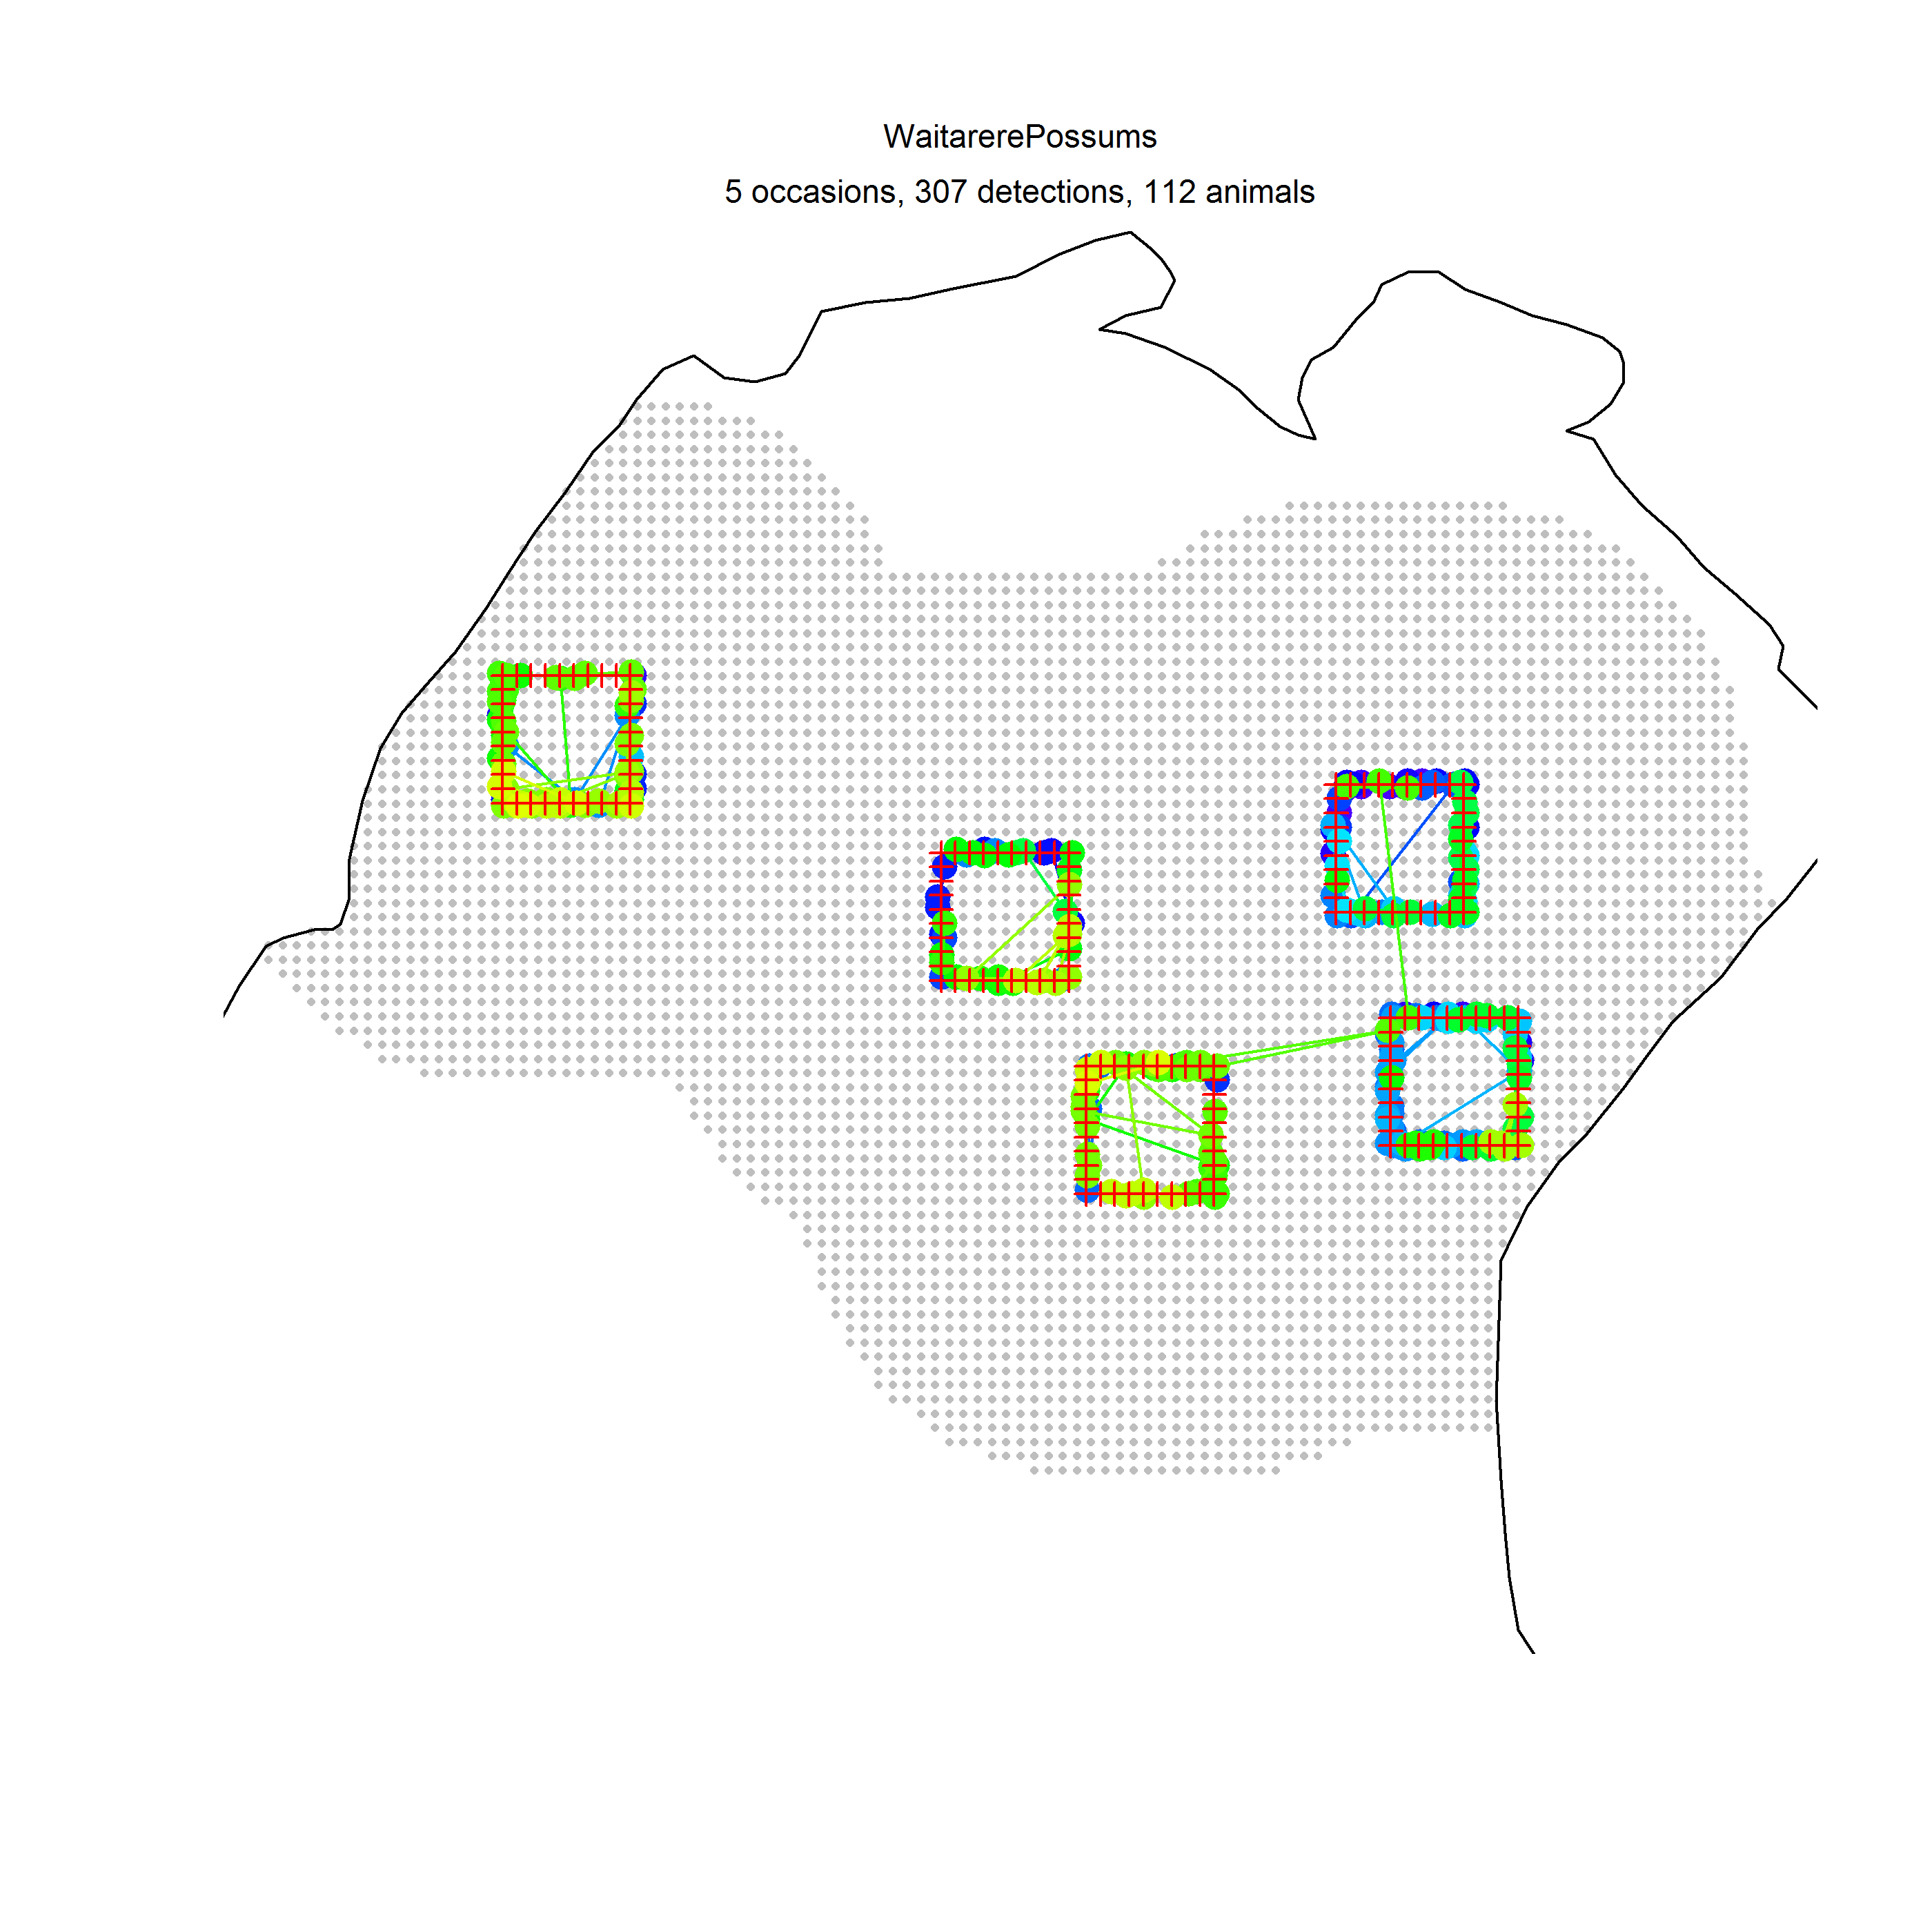
\includegraphics[width=5in]{Ch9-PoisMn/figs/possum.png}
\caption{Trapping grids used in possum study from
  \citet{efford_etal:2005}, data are contained in the \R
package \mbox{\tt secr}
\citep{efford:2011}, refer to the help file \mbox{\tt ?possum} for
additional details of this study.}
\label{poisson-mn.fig.possum}
\end{figure}

The data file \mbox{\tt possumCH} contains 112 encounter histories,
and we analyze those here although the last 8 of those are recaptures
treated as new individuals\footnote{M. Efford, personal communication}.
%Trapping produced
%46 adult females, 33 adult males, 10 immature females and 11
%immature males; sex and/or age were not recorded for 4 individuals
%(M. Coleman unpubl. data).
The encounter process is not strictly a single-catch multinomial process because,
as noted in the \mbox{\tt possum} help file
 ``One female possum was twice captured at two
sites on one day, having entered a second trap after being released;
one record in each pair was selected arbitrarily and discarded.''
which is a similar situation to what might happen in bird mist net
studies, as a bird might fly into a net upon release from another.
By discarding the two
extra-capture events, we can satisfactorily view these data as
single-catch data, for which \mbox{\tt secr} uses the independent
multinomial likelihood (M. Efford, pers. comm.).
If multiple, same-session captures 
were common, then it might be worth developing a 
model for $n_{ik} = $ the number of captures of individual $i$ during
sample occasion $k$, in order to make use of all captures. 

For our Bayesian analysis here, we used a rectangular state-space which
doesn't account for any geographic boundaries of the survey region, but
we note that a habitat mask is included in {\tt secr} and it could be
used in a Bayesian analysis.
%, and we analyze the
%data using that mask in Chapt. \ref{chapt.mle}.
Whether or not we use the mask is
probably immaterial as long as we understand the predictions of $N$ or
$D$ over the water don't mean anything biological and we probably
wouldn't report such predictions. 
 The {\bf JAGS} model
specification is based on that of the ovenbird analysis given
previously, and so we don't reproduce the model here. The {\bf R/JAGS}
script is called \mbox{\tt SCRpossum},  which is in the \mbox{\tt scrbook}
package.
The results are summarized in Table \ref{poisson-mn.tab.possum}.



\begin{table}[ht]
\centering
\caption{Results of fitting the independent multinomial observation
 model to the possum trapping data. Strictly speaking, the trapping
  device is a ``single-catch'' trap, and the model represents an intentional
  misspecification. Density is reported in individuals per ha ($Dha$).
Posterior summaries were obtained using {\bf JAGS} with
 3 chains, each with 2000 iterations, discarding the first 1000 as
 burn-in, to yield a total of 3000 posterior samples.
}
\begin{tabular}{crrrrrrr} \hline \hline
 Parameter & Mean &  SD   & 2.5\% & 50\%  & 97.5\% &Rhat& n.eff \\ \hline
%D        &  0.000 &  0.000&   0.000 &  0.000 &  0.000 &1.009 &  340\\
N        & 235.407&  17.435& 204.000& 235.000& 270.000& 1.009&   340\\
Dha      & 1.549  &  0.115&   1.343 &  1.547 &  1.777 &1.009 &  340\\
$\alpha_0$   &-0.935  &  0.167 & -1.270 & -0.934 &  -0.605& 1.007&   870\\
$\alpha_1$   &0.000   & 0.000  & 0.000  & 0.000  &   0.000& 1.001&  2800\\
$\psi$      &0.783   & 0.062  & 0.666  & 0.782  &   0.903& 1.008&   340\\
$\sigma$   &52.020   & 2.675  &47.067  & 51.933 &  57.585& 1.001&  2800
\\ \hline
\end{tabular}
\label{poisson-mn.tab.possum}
\end{table}


The estimated density (posterior mean) is about 1.53 possums/ha.
To obtain the \mbox{\tt secr} results for the equivalent null model, we execute the following command
\begin{verbatim}
> secr.fit( capthist = possumCH, trace = F )
\end{verbatim}
which produces (edited) summary output:
\begin{verbatim}
[... some output deleted ...]

Fitted (real) parameters evaluated at base levels of covariates
       link   estimate SE.estimate        lcl        ucl
D       log  1.6988930  0.17352645  1.3913904  2.0743547
g0    logit  0.1968542  0.02256272  0.1563319  0.2448321
sigma   log 51.4689114  2.59981905 46.6204139 56.8216500

[... some output deleted ...]
\end{verbatim}
As we've discussed previously, there are many reasons for why there
might be differences between Bayesian and likelihood estimates.  But
even among likelihood estimates -- any time you run a model there is
some numerical integration going on which requires some specific
choices of how to do the integration (see Chapt. \ref{chapt.mle}).
For now we just observe that the estimated density is certainly in the
ballpark (compared to those in Table. \ref{poisson-mn.tab.possum}), and so too is the estimated $\sigma$.

%%%{\bf XXX RERUN WITH LARGER STATE SPACE XXXX}
%%%%{\bf XXXX TO DO XXXXXX Density MAP XXXXXX}


\section{Acoustic sampling}
\label{poisson-mn.sec.acoustic}

The last decade has seen an explosion of technology that benefits the
study of animal populations. This includes DNA sampling methods that
allow for identification from hair or scat, camera trapping and
identification software that allow efficient sampling of many
mammals, and the resulting statistical technology that helps us to
make sense of such data \citep{borchers_efford:2008,
  royle_young:2008,efford_etal:2009ecol, gopalaswamy_etal:2012ecol,
  sollmann_etal:2012ecol, chandler_royle:2012}.  One other extremely
promising technology area is that of acoustic sampling using
microphones or recording devices.  That is, instead of having cameras
record encounters, or humans pick up scat, we can establish an array of
(usually) electronic recording devices which, instead of establishing
a visual identity of individuals, record a vocal expression of
each individaul.  In this context, \citet{efford_etal:2009ecol}
referred to audio recorders as ``signal strength proximity detectors''
to distinguish them from other types of proximity detections,
including camera traps, which are {\it visual} proximity detector.
Using audio records, the spatial pattern of the {\it signal strength}
at the different audio recorders or microphones can be used for inference about density
\citep{dawson_efford:2009,efford_etal:2009ecol} in the same way as the
spatial pattern of detections is used in the types of SCR models we
have discussed so far.
% XXXX Here you might say that an important distinction is that
% density in this case is "sound sources"
% per area, rather than activity centers per area.
The basic technical formulation of these
models comes from \citet{efford_etal:2009ecol}, and it was applied to
field study of birds by \citet{dawson_efford:2009}. In that study,
recording devices were organized in groups of 4 (in a square pattern),
% XXXX plot(signalCH) makes it look like a square pattern
% ok
with an array of $5 \times 15$ such clusters of 4, seperated by 100 m
(300 total recorder locations).  This data set,
called \verb+signalCH+, % XXXX
is provided with the
\mbox{\tt secr} package along with some sample analyses and help
files.
See \citet{efford_dawson:2010}, a version of the document
\mbox{\tt secr-sound.pdf} (that also comes with the \mbox{\tt secr} package)
which you can access directly from the main help file (\mbox{\tt
  ?secr}).

Our development here mostly follows \citet{efford_etal:2009ecol}, but
we change some notation to be consistent with our previous material.
Let $S({\bf x}, {\bf u})$ be the strength of a signal emanating from
signal 
location ${\bf u}$, as recorded by a device at location ${\bf
  x}$. 
Just as ordinary SCR models represent a model of {\it encounter
  frequency} as a function of distance, in acoustic models, the
acoustic SCR model is a model of sound attenuation as a function of
distance.  In particular, the acoustic models assumes that $S$ (or a
suitable transformation) declines with distance $d$ from the origin of
the sound, to the recording device. In the context of spatial sampling
of animals, the origin is the actual location of some individual
animal, and the recording device is something we nailed to a tree, or
mounted on a post.  For example, a model of sound
attenuation used by \citet{dawson_efford:2009} is the following:
\begin{equation}
S({\bf x},{\bf u})  = \alpha_{0} + \alpha_{1} d({\bf x},{\bf u}) +
\epsilon
\label{poisson-mn.eq.signal}
\end{equation}
% XXXX Does epsilon need a subscript?
% technically it hsould have an x, u index also -- but I think we'll 
% leave it off and just call it "iid noise" for simplicity
where $\epsilon \sim \mbox{Normal}(0, \sigma_{s}^{2})$. In many standard
situations, $S$ will be measured in decibels, which can be any value
on the real line.  In the conduct of acoustic sampling and the
development of custom models for your own situation, it would probably
be helpful to know something about sound dynamics and signal
processing.  In this model, the
parameters $\alpha_0$, $\alpha_1$ and $\sigma_{s}^{2}$ are to be
estimated. We abbreviate the set of parameters by $\bm \theta$ for short.

The basic structure of an acoustic SCR study is not really much different from
ordinary SCR studies.
Just as ordinary SCR models require that individuals be
encountered at $>1$ trap, these acoustic models require that
individuals be heard at $>1$ recorder. Therefore, 
the acoustic signals (calls or vocalizations) must be 
 reconcilable and, in fact, reconciled successfully by the
investigator. In practice, this would require associating signals that
occur at the same instant with the same individual (or making a
decision one way or the other). Further, if individuals are actively
moving during the sample period (that recorders are functioning) then
individuals might be double-counted, thereby biasing estimates of
density. In general, the models produce an estimate of density of {\it
  sources}, and how that is interpreted depends on whether individuals
are stationary or mobile, and other things. 
In particular, if multiple survey occasions are
used (e.g., on different days), then modeling movement of individuals
would be essential in order to interpret estimates of density
meaningfully. 
Models that allow some
movement should be possible (see Sec. \ref{acoustic.bugs} below, and
Chapts.  \ref{chapt.search-encounter} and
\ref{chapt.open}). 


\subsection{The signal strength model}

We assert that an individual is detected if $S$ exceeds a threshold,
$c$. The reason for introducing this threshhold $c$ is that sound
recorders will always record some
background 
sound, and so effective use of the
acoustic SCR models requires specification of the threshold of
measured signal below which the record is censored (non-detection
occurs) because the recorded sound it assumed to be background noise.
So we assert that an individual is detected if $S>c$ which occurs with
probability $\Pr(S > c)$, the encounter probability.  To expand on and
formalize this, let $S_{ij}$ be the observed value of $S$ for animal $i$ at
detector $j$.  The encounter probabiliy is $\Pr(S_{ij}>c)$ which is
$\Pr(S_{ij}>c) = 1- \Pr(S_{ij} < c)$, so that, if we standardize the
variate we have
\[
1-\Pr\left( \frac{ (S_{ij}- \mathbb{E}(S))}{\sigma_{s}}  <  \frac{
(c -  \mathbb{E}(S)) }{\sigma_{s}} \right)
\]
This probability % XXXX This sentence is somewhat hard to follow
calculation requires evaluation of the CDF  of a standard normal variate
say, $\eta = (S_{ij}- \mathbb{E}(S))/\sigma_{s}$, being
less than 
$\gamma({\bm \theta}) = (c -  \mathbb{E}(S))/\sigma_{s}$, 
which is a function of all the parameters $\alpha_{0}$, $\alpha_{1}$,
$\sigma_{s}^{2}$ and also the individual location ${\bf u}$ and trap location
${\bf x}$.
We'll identify it by
$\gamma({\bm \theta},{\bf x},{\bf u})$ when we need to be explicit
about those things.
 We can compute
$\Pr(S_{ij}>c) = 1-\Pr(  \eta <
\gamma({\bm \theta}, {\bf x},{\bf u}))$ easily using any software
package including {\bf R} which has a standard function, \mbox{\tt
  pnorm}, for computing the normal cdf.
To be more precise, we'll use the $\Phi()$ to represent the normal
cdf. Therefore, an individual is encountered whenever $S_{ij}>c$ which
happens with probability
$\Pr(S_{ij}>c) = 1-\Phi( \gamma({\bm \theta}, {\bf x},{\bf u}) )$.

Naturally this quantity should depend on {\it where} an individual is
located at the time of recording
-- what we call it's instantaneous location, say ${\bf u}$, to
distinguish it from it's
 home-range center ${\bf s}$ (but we outline a model below that
 contains both ${\bf u}$ and ${\bf s}$),
and also the trap ${\bf x}$, so we
 index the quantity $\gamma$ by those two quantities, in
addition to the parameters $\alpha_{0}$, $\alpha_{1}$ and $\sigma_{s}$.
The probability of detection is therefore
\[
p_{ij} = p(\alpha_0, \alpha_1, \sigma | {\bf x}_{j}, {\bf u}_{i} ) = 1- \Phi( \gamma(\cdot))
\]
where
 ${\bf u}_{i}$ is the instantaneous location of individual $i$ and
${\bf x}_{j}$ is the location of trap $j$.  We'll suppose here that
the random variables ${\bf u}_{i}$ have state-space ${\cal
  U}$\footnote{We use ${\cal U}$ here to avoid confusion with
  definition of signal strength, $S$. However, ${\cal U}$ is the same
  state-space as ${\cal S}$ in the rest of the book}.

How do we interpret this probability? Well, two things have to happen
for an individual to be encountered by a trap:
(1)  it has to  vocalize; (2)
the microphone has to record a signal $>c$. These two things
together are a product of biological and environmental factors which
could include time of day, wind direction and speed, or maybe rain,
humidity and other things. The bottom line is a lot of factors are
balled up in whether or not the microphone records a sound greater
than the threshhold.  

The observations from an acoustic survey are the signal strength
measurements, and
the likelihood of the observed signal strength
from individual $i$ at detection
device $j$ can be specified by noting that
the
likelihood is the normal pdf for the observed signal {\it if} the
signal strength is $>c$ and, otherwise, the contribution to the
likelihood is $\Phi(\gamma(\cdot))$ (see Eq. 8 of \citet{efford_etal:2009ecol}):
\[
\Pr(S_{ij}| {\bf u}_{i} ) = \Phi( \gamma( \cdot) )^{1-1(S_{ij}>c)}
\mbox{Normal}(S_{ij};\alpha_{0},\alpha_{1},\sigma_{s},{\bf x}_{j},{\bf
u}_{i})^{1(S_{ij}>c)}
\]
\begin{comment}
XXXX Note: I think this formula is wrong. Why shouldn't this be a
  truncated-Normal PDF? XXXXXX i.e., $Pr(S|S>c)$? It should be, but
  then by ``capturing'' the guy, this happens with probability Pr(S>c)
and so that cancels from the denominator.
i.e., the likelihood is really:
Pr(S|S>c and S>c) =
[ Pr(S)/Pr(S>c) ] * Pr(S>c)    = Pr(S)

I don't think Efford et al. explained the origins of this formula very well!
\end{comment}

We can use this as the basis for constructing the binomial-form of the
likelihood as we did in Chapt. \ref{chapt.mle}, which involves the
number of individuals not encountered, $n_{0}$.  The probability that
an individual is {\it not} captured is equal to the probability that
its signal strength doesn't exceed $c$ at any microphone.  The
probability of not being captured at a microphone ${\bf x}_{j}$ is:
\[
1-p_{{\bf u},j} = \Phi( \gamma(\cdot) )
\]
and therefore the probability of not being captured at any microphone is:
\[
\Pr(\mbox{all } S_{{\bf u},j} < c | {\bf u}) = \prod_{j=1}^{J} ( 1-p_{{\bf u},j} )
= \prod_{j=1}^{J} \Phi( \gamma(\cdot, {\bf x}_{j}, {\bf u}) )
\]
and therefore the marginal probability of not being captured is
\[
\pi_{0} = [ \mbox{all }  S_{{\bf u},j} < c | {\bm \alpha}] =
\int_{{\cal U}}
 \left\{
\prod_{j=1}^{J} \Phi( \gamma( {\bm \theta}, {\bf x}_{j}, {\bf u}) )
 \right\}
 d{\bf u}
\]
which can be used to construct the binomial form of the likelihood as
we did in Chapt. \ref{chapt.mle} (see Eq. \ref{mle.eq.binomialform}).




\begin{comment}


The probability that signal strength exceeds ``c'' at one or more
detectors is:
\begin{verbatim}
p_{dot}(X) = 1- \prod_{k=1}^{K}(   1-\phi(  gamma(X,k)) )
\end{verbatim}

\end{comment}

\subsection{Implementation in \mbox{\tt secr}}

Fitting acoustic encounter models in \mbox{\tt secr} is no more
difficult than other SCR models. There is a handy manual (\mbox{\tt
  secr-sound.pdf}) with examples \citep{efford_dawson:2010} which
comes with the \mbox{\tt secr} package.  The basic process is that
\mbox{\tt make.capthist} will make a \mbox{\tt capthist} object from a
3-dimensional 
encounter array -- which is a binary array indicating whether each
individual was detected or not at each recorder/microphone. In the
case of signal strength data, \mbox{\tt secr} handles the case  where \#
occasions = 1, i.e., the recorders obtained
data for a single sample occasion, but this is not a general requirement of the
model for signal strength data (see next section).  The ``signal'' attribute of the \mbox{\tt
  capthist} object contains the signal strength in decibels.  The best
way to include the signal attribute is to use \mbox{\tt make.capthist}
in the usual way, providing it with the encounter data and trap data
and, in addition, the variable ``cutval'' (which is $c$ in our
notation above) and then provide the signal strength data as an extra
column of the \mbox{\tt capthist} object.  See \mbox{\tt
  ?make.capthist} for details.
\begin{comment}
``Signal strengths may be
provided in the fifth (fmt = trapID) or sixth (fmt = XY)
columns. Detections with signal strength missing (NA) or below
'cutval' are discarded.''

The ``ovensong'' data set in \mbox{\tt secr} has an example (\mbox{\tt
  ?ovensong}) which is from \citep{dawson_efford:2009}.

You have to set the \mbox{\tt cutval}..... which we called $c$ above.
Otherwise fitting a model in \mbox{\tt secr} goes the same as for any
other model. For the \mbox{\tt ovensong} example in \mbox{\tt secr}
has the following code:


## apply signal threshold
signalCH.525 <- subset(signalCH, cutval = 52.5)

## Not run:
## models with and without spherical spreading
omask <- make.mask(traps(signalCH), buffer = 200)
ostart <- c(log(20), 80, log(0.1), log(2))
ovensong.model.1 <- secr.fit( signalCH.525, mask = omask,
    start = ostart, detectfn = 11 )
ovensong.model.2 <- secr.fit( signalCH.525, mask = omask,
    start = ostart, detectfn = 10 )

\end{comment}



\subsection{Implementation in {\bf BUGS}}
\label{acoustic.bugs}

We don't know of any Bayesian applications of acoustic SCR models,
although we imagine that implementation of such models in the {\bf
  BUGS} engines should be achievable.  It seems easy enough to write
down a general hierarchical model that would accomomdate sampling on
repeated occassions. Let ${\bf s}_{i}$ be the home range center, and
let ${\bf u}_{ik}$ the instantaneous location of individual $i$ during
sample occasion $k$ (see Chapt. \ref{chapt.search-encounter} for
similar models). The model for ${\bf u}_{ik}$ can be specified
conditional on ${\bf s}_{i}$. For example, we could assume that ${\bf
  u}_{ik}$ are bivariate normal draws with mean ${\bf s}_{i}$ and some
variance $\sigma_{u}^{2}$. Then, conditional on ${\bf u}_{ik}$ an
individual produces a signal according to the signal attenuation model
(Eq. \ref{poisson-mn.eq.signal}), or perhaps some other model. Then we
generate the binary encounter data by truncating the observed signal
at $c$. This general model then is an example of an SCR model in which
parameters of a movement model are identifiable
(see Sec. \ref{modeling.sec.characterization})
 because
there is direct information about movement outcomes from the sampling
method, unlike other types of encounter methods (e.g., camera traps)
for which animal locations are restricted to a set of fixed, pre-determined
points where traps are located.  Other types of SCR methods allow for
movement information too, including some of the search-encounter
models (Chapt. \ref{chapt.search-encounter}).


Instead of developing a Bayesian version of this model here,
we leave it to the reader to
explore simulating data and devising a Bayesian implementation of the
acoustic model in one of the {\bf BUGS} engines.
% XXXX I wonder if we could show some generic BUGS code for this,
% without supplying simulated data? Below is a hack at this:
Note that for a
single occasion, you can simulate the data using the two stage model
(having both ${\bf s}$ and ${\bf u}$) or you can simulate ${\bf u}$
uniformly without dealing with ${\bf s}$ in the model.
The kernel of the {\bf BUGS} model specification 
should resemble the following snippet:
{\small
\begin{verbatim}
model {
  # ignoring loops and data augmentation
  u[i,1] ~ dunif(xlim[1], xlim[2])
  u[i,2] ~ dunif(ylim[1], ylim[2])
  mu[i,j] <- alpha0 + alpha1*d[i,j]
  ###
  ###  JAGS has this T() truncation feature
  S[i,j] ~ dnorm(mu[i,j], 1/sigma^2)T(c,Inf) 
  ###
  gamma[i,j] <- (c - mu[i,j])/sigma
  p[i,j] <- 1 - pnorm(gamma[i,j], 0, 1) # JAGS has pnorm() function
  y[i,j] ~ dbern(p[i,j])
}
\end{verbatim}
}



\begin{comment}
  XXXX It seems like there are a lot of general considerations that
  the practitioner will need to think about. For example, these
  acoustic models assume that the survey is conducted during an
  ``instant'' in time right? You offered a way of dealing with
  movement, but what if a bird sings twice during a time interval?
  If they are different songs, wouldn't this model incorrectly think
  that they are two distinct birds?

  Another biggie is how do you interpret this density estimate? It
  doesn't account for the probability that an individual vocalizes
  right? Don't we somehow need an estimate of that if we want
  animals/area instead of sounds/area? I don't think alpha0 can be
  interpretted in this way, right?

  I guess Dawson and Efford get at some of this in their abstract, where
  they say ``The method requires that
  individuals detected at the same place are acoustically
  distinguishable and all individuals vocalize
  during the recording interval, or that the per capita rate of
  vocalization is known.'' We should probably mention this.

  Two other things: (1) We need to briefly discuss ``spherical
  spreading''. D and E say this about Eq1: The second term describes the spherical spread of sound energy,
and the final term represents log-linear attenuation from all other
causes (b1 < 0).We set lS = b0 for d < 1,when spherical spreading
generally does not apply (Wiley & Richards 1982), thus avoiding
computational problems at d = 0.

And (2) we need to cite some of Tiago's papers on this stuff.
\end{comment}


\subsection{Other types of acoustic data}

\citet{efford_dawson:2010} noted that various other types of acoustic
data might arise for which SCR-like models would be
useful\footnote{Some of the following is also related to material
  presented by D.L. Borchers at the ISEC 2012 conference in Norway.}.
For example, we could measure the {\it time of
  arrival} of a vocal queue of some sort at multiple recorders to
estimate the number and origin of $N$ queues.
Another example is that where we measure {\it direction} to a queue
from multiple devices and do, effectively, a type of statistical
triangulation to the multiple but unknown number of sources.  This has
direct relevance to types of double or multiple-observer sampling that
people do in field studies of birds. Normally 2 observers stand in
close proximity and record birds, reconciling their detections after
data collection. An SCR-based formulation of the double-observer
method has two observers (or more) standing some distance apart, e.g.,
50 or 100 meters,  and marking individual birds on a map (or at
least a direction) and a time of detection.  The SCR/double-observer
method could be applied to such data.



\section{Summary and Outlook}

In this chapter we extended SCR models to accommodate alternative
 models for the observation process, including Poisson and multinomial models.  Along
with the binomial model described in Chapt. \ref{chapt.scr0}, this
sequence of models will accommodate a substantial majority of
contemporary spatial capture-recapture problems, including
the 4 main types of encounter data:
binary encounters, multinomial trials from ``multi-catch'' and
``single-catch'' \citep{efford:2004, efford:2011, royle_gardner:2011}
trap systems, and Poisson encounter frequency data from devices that can
record multiple encounters of the same individual at a device.  We
summarize the standard observation models and the corresponding
\mbox{\tt secr} terminology in Table \ref{poisson-mn.tab.models}.  What
we refer to as search-encounter (or area-search) models (see
Chapt. \ref{chapt.search-encounter}) are distinct
from most of the other classes in that the observation location can
also be random (in contrast to traps, where the location is fixed by
design). This auxiliary data is informative about an intermediate
process related to movement \citep{royle_young:2008}.

\begin{table}[ht]
\centering
\caption{
Different observation models, where we discuss then in this
  book, and what the corresponding \mbox{\tt secr} terminology is
}
\begin{tabular}{lll}
\hline \hline
observation model & Where in this book?  &  \mbox{\tt secr} name  \\ \hline
Bernoulli         & Chapt. \ref{chapt.scr0}    &   \mbox{\tt proximity} \\
Poisson           & Sec. \ref{poisson-mn.sec.poisson} & \mbox{\tt count} \\
Multinomial (ind) & Sec. \ref{poisson-mn.sec.multinomial} & \mbox{\tt  multi-catch} \\
Multinomial (dep) & Sec. \ref{poisson-mn.sec.singlecatch} & \mbox{\tt  single-catch} \\
Acoustic          & Sec. \ref{poisson-mn.sec.acoustic}
   &  \mbox{\tt signal}  \\
Search-encounter      & Chapt. \ref{chapt.search-encounter}  &
\mbox{\tt polygon} (in part) \\ \hline
\end{tabular}
\label{poisson-mn.tab.models}
\end{table}

There is a need for other types of encounter models that arise in practice. We
identify a few of them here, although we neglect a detailed
development of them at the present time or, in some cases, put that
off until later chapters: (1) Removal systems -- Sometimes traps kill
individuals and SCR models can handle that. This can be viewed as a
kind of open model, with mortality only, and we handle such models (in
part) in % XXXX Except, no recaptures can occur, so this seems
         % impossible in SCR. Or, it seems like an interesting
         % research avenue.
Chapt. \ref{chapt.open};  (2) There are models for which only specific
summary statistics are observable
\citep{chandler_royle:2012,sollmann_etal:2012ecol} which we cover in
Chapts. \ref{chapt.scr-unmarked} - \ref{chapt.partialID}; (3) We can
have multiple observation methods working together as in
\citet{gopalaswamy_etal:2012ecol}.

There remains much research to be done to formalize models for certain
observation systems. For example, while we think one will usually be
able to analyze single-catch systems using the multi-catch model, or
even the Bernoulli model if encounter probability is sufficiently low,
a formalization of the single-catch model would be a useful
development and, we believe, it should be achievable using one or
another of the {\bf BUGS} engines.  In addition, classical ``trapping
webs'' \citep{anderson_etal:1983, wilson_anderson:1985b,
  jett_nichols:1987, parmenter_etal:1989,link_barker:1994}
have been around for quite
some time and it seems like they are amenable to formulation as a type
of SCR model although we have not pursued that development simply
because trapping webs are rarely used in practice.

